 \documentclass[a4paper,twosided, 15pt]{book}
%\usepackage[czech]{babel}
\usepackage[utf8]{inputenc}
\usepackage{listings}
\usepackage[T1]{fontenc}
\usepackage{float}
\usepackage{graphicx}
\usepackage{makeidx}
\usepackage{fancyhdr}
\usepackage{longtable}
\usepackage[usenames,dvipsnames]{color}
\usepackage{pifont}
\usepackage{wrapfig}
\usepackage[footnotesize,bf]{caption}
\usepackage[colorlinks=true,linkcolor=blue,urlcolor=blue,pdftitle=MDS manual,pdfsubject=yyy,pdfkeywords=zzz,pdfauthor=Martin Madron,bookmarksopen=false,pdfpagemode=None]{hyperref}
    %\usepackage{underscore}
%\setcounter{chapter}{0} 0x0xxxxx

% \setcounter{chapter}{0} 0x0xxxxx

%\setcounter{chapter}{-1}
\floatstyle{ruled}
\newfloat{code}{thp}{lop}
\floatname{code}{Code}

\definecolor{highlight_constant}{rgb}{0.333, 0.666, 0.0}
\definecolor{highlight_unknown_base}{rgb}{0.533, 0.133, 0.133}
\definecolor{highlight_comment}{rgb}{0.533, 0.533, 0.533}
\definecolor{highlight_symbol}{rgb}{0.666, 0.0, 1.0}
\definecolor{highlight_oper_sep}{rgb}{0.866, 0.533, 0.0}
\definecolor{highlight_directive}{rgb}{0.533, 0.533, 1.0}
\definecolor{highlight_label}{rgb}{0.533, 0.333, 0.0}
\definecolor{highlight_instruction}{rgb}{0.0, 0.0, 1.0}
\definecolor{highlight_sfr}{rgb}{0.0, 0.0, 0.866}
\definecolor{highlight_indirect}{rgb}{0.866, 0.0, 0.0}
\definecolor{highlight_imm_hex}{rgb}{0.666, 0.0, 0.866}
\definecolor{highlight_macro}{rgb}{0.8, 0.0, 0.866}
\definecolor{highlight_imm_dec}{rgb}{0.0, 0.533, 0.866}
\definecolor{highlight_hex}{rgb}{0.533, 0.0, 0.733}
\definecolor{highlight_oct}{rgb}{0.533, 0.0, 0.0}
\definecolor{highlight_dec}{rgb}{0.0, 0.333, 0.666}
\definecolor{highlight_bin}{rgb}{0.2, 0.2, 0.333}
\definecolor{highlight_string}{rgb}{0.533, 0.533, 0.0}
\definecolor{highlight_control}{rgb}{1.0, 0.0, 0.0}
\definecolor{highlight_imm_oct}{rgb}{0.666, 0.0, 0.0}
\definecolor{highlight_imm_bin}{rgb}{0.333, 0.333, 0.666}
\definecolor{highlight_char}{rgb}{0.0, 1.0, 1.0}
\definecolor{highlight_imm_constant}{rgb}{0.937, 0.737, 0.168}
\definecolor{highlight_imm_unknown}{rgb}{0.666, 0.2, 0.2}
\definecolor{highlight_lst_number}{rgb}{0.0, 0.882, 1.0}
\definecolor{highlight_lst_code}{rgb}{1.0, 0.2, 0.968}
\definecolor{highlight_lst_address}{rgb}{0.349, 0.356, 1.0}
\definecolor{highlight_lst_line}{rgb}{0.074, 0.003, 0.513}
\definecolor{highlight_lst_macro}{rgb}{0.533, 0.533, 0.533}
\definecolor{highlight_lst_include}{rgb}{0.533, 0.533, 0.533}
\definecolor{highlight_lst_msg}{rgb}{0.0, 0.0, 0.0}
\newcommand{\menuitem}[1]{\texttt{#1}}
\newcommand{\fileextension}[1]{\texttt{#1}}
\newcommand{\mysmallfont}{\fontsize{8pt}{10pt} \selectfont{}}
\newcommand{\uC}{$\mu$C }

\pdfadjustspacing=1
\raggedbottom

\makeindex
\pagestyle{fancy}
\fancyhf{}
\fancyhead[EL,OR]{\bfseries\thepage}
\fancyhead[LO]{\bfseries\rightmark}
\fancyhead[RE]{\bfseries\leftmark}

\fancypagestyle{plain}{
	\fancyhead{}
	\fancyhead[EL,OR]{\bfseries\thepage}
	\renewcommand{\headrulewidth}{0pt}
}


%%%%%%%%%%%%%%%%%%%%%%%%%%%%%%%%%%%%%%%%%%%%%%%%
 %%%%%%%%%%%%%%%%%%%%%%%%%%%%%%%%%%%%%%%%%%%%%%%%%%%%%%%
\title{Multitarget Development Environment \\
2013/2014}
\author{Moravia Microsystems s.r.o \\}

%%%%%%%%%%%%%%%%%%%%%%%%%%%%%%%%%%%%%
\begin{document}
\maketitle

        \begin{center}
        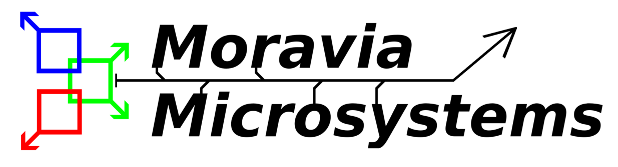
\includegraphics[scale=0.1]{img/Moravia_Microsystems.png}
        \end{center}


\newpage
\tableofcontents
\newpage

\chapter{Preface}
\index{This manual} is an \index{introduction} to the \index{Moravia Microsystems} development tools designed for microcontrollers.
It introduces the MDS Integrated Development Environment, Simulator and
presents a step-by-step guided tour of the numerous features and capabilities
the Moravia Microsystems embedded development tools offer.

\chapter{About MDS}
MDS is a window-based software development platform that
combines a robust and modern editor with a project manager
and make facility tool. It integrates all the tools needed
to develop embedded applications including a C/C++ compiler, macro
assembler, linker/locator, and a HEX file generator. MDS helps
expedite the development process of embedded applications by providing
the following:
        \section{Features}
                \begin{itemize}
                    \item Full-featured source code editor
                    \item Project Manager for creating and maintaining your projects
                    \item Integrated Make Utility functionality for assembling, compiling, and linking your embedded applications
                    \item Test bench - Displays changes of values on a time graph. Study the signal and variable changes and view their dependency. Simulates all possible outside conditions
                \end{itemize}

	\section{Requirements}

\chapter{Quick start}
        \section{Demonstration project}
        The aim of the demonstration project is to provide an easy way to explore
        the IDE without reading long documents. The
        demonstration project can be opened from the welcome dialog ( Main Menu
        Help Welcome dialog Open demonstration project. )
        Demonstration project should introduce new user into usage of the most
        common functions of the IDE like assembling the code, running simulator
        and so on. Demonstration project cannot be modified by the user in order
        to make it less volatile.
                \begin{figure}
                    \centering{}
                    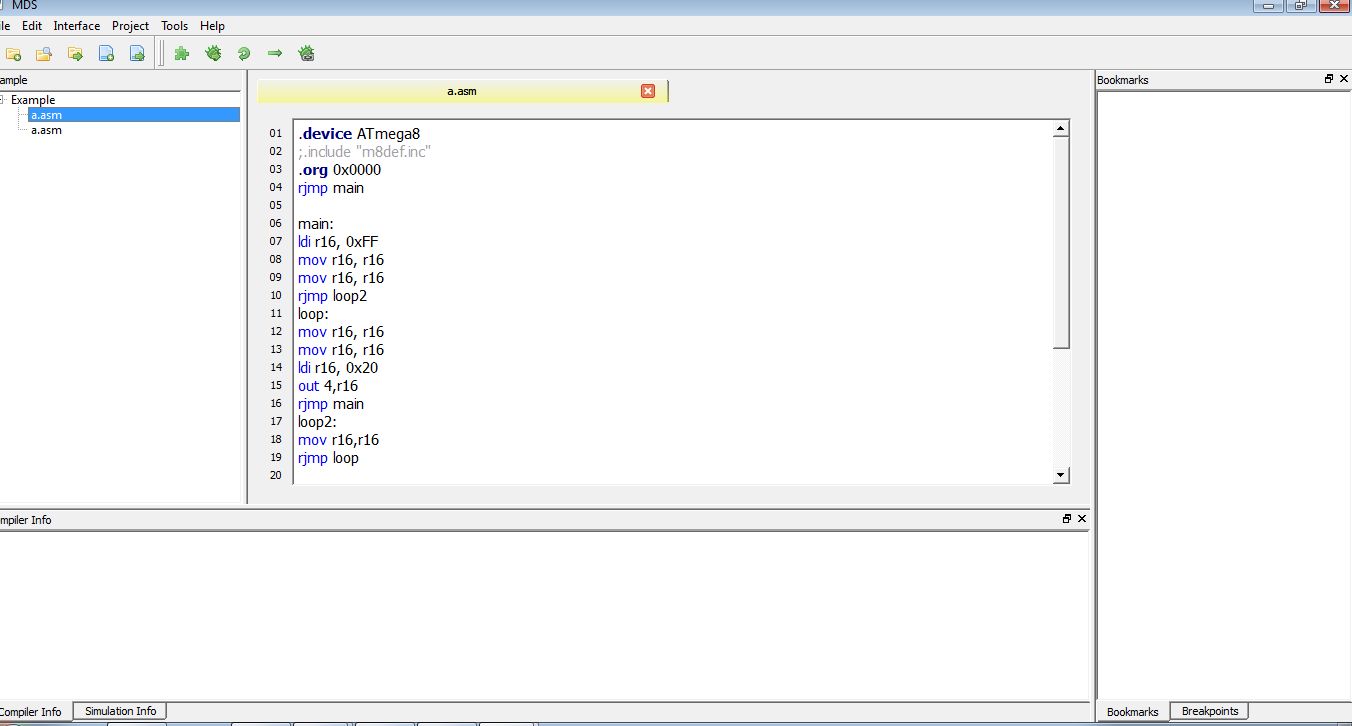
\includegraphics [scale=0.4]{img/Demonstration_project.png}
                    \caption{Demonstration project}
                \end{figure}
        \section{Your first project}

        \section{What is PicoBlaze?}
        PicoBlaze is the designation of a series of three free soft processor cores
        from Xilinx for use in their FPGA and CPLD products. They are based on a RISC
        architecture of 8 bits and can reach speeds up to 100 MIPS on the Virtex 4
        FPGA"s family. The processors have an 8-bit address and data port for access
        to a wide range of peripherals. The license of the cores allows their free
        use, albeit only on Xilinx devices, and they come with development tools.
        All instructions execute in two clock cycles, making performance of the core instruction
        set deterministic. Interrupt response is not more than five clock cycles. As a resource
        optimization, it is possible for two PicoBlaze cores to share the same 1k x 18 instruction
        PROM, taking advantage of the dual-ported implementation of this block on Xilinx FPGAs.

                \subsection{PicoBlaze features:}
                        \begin{itemize}
                                \item 16 byte-wide general-purpose data registers
                                \item 1K instructions of programmable on-chip pr
                                        ogram store, automatically loaded during
                                        FPGA configuration
                                \item Byte-wide Arithmetic Logic Unit (ALU) with CARRY and ZERO indicator flags
                                \item 64-byte internal scratchpad RAM
                                \item 256 input and 256 output ports for easy expansion and enhancement
                                \item Automatic 31-location CALL/RETURN stack
                                \item Predictable performance, always two clock cy
                                        cles per instruction, up to 200 MHz or
                                        100 MIPS in a Virtex-II Pro FPGA
                                \item Fast interrupt response; worst-case 5 clock cycles
                                \item Optimized for Xilinx Spartan-3, Virtex-II, and Virtex-II Pro FPGA architectures just
                                        96 slices and 0.5 to 1 block RAM
                                \item Assembler, instruction-set simulator support
                        \end{itemize}

\chapter{User interface}
         \section{Window Layout Concept}
          Developers can define their working environment to fit the needs and
          preferences. For a better understanding of further comments and instructions,
          five major screen areas are defined. % pops�no v obr�zku
               \begin{figure}
                      \centering
                      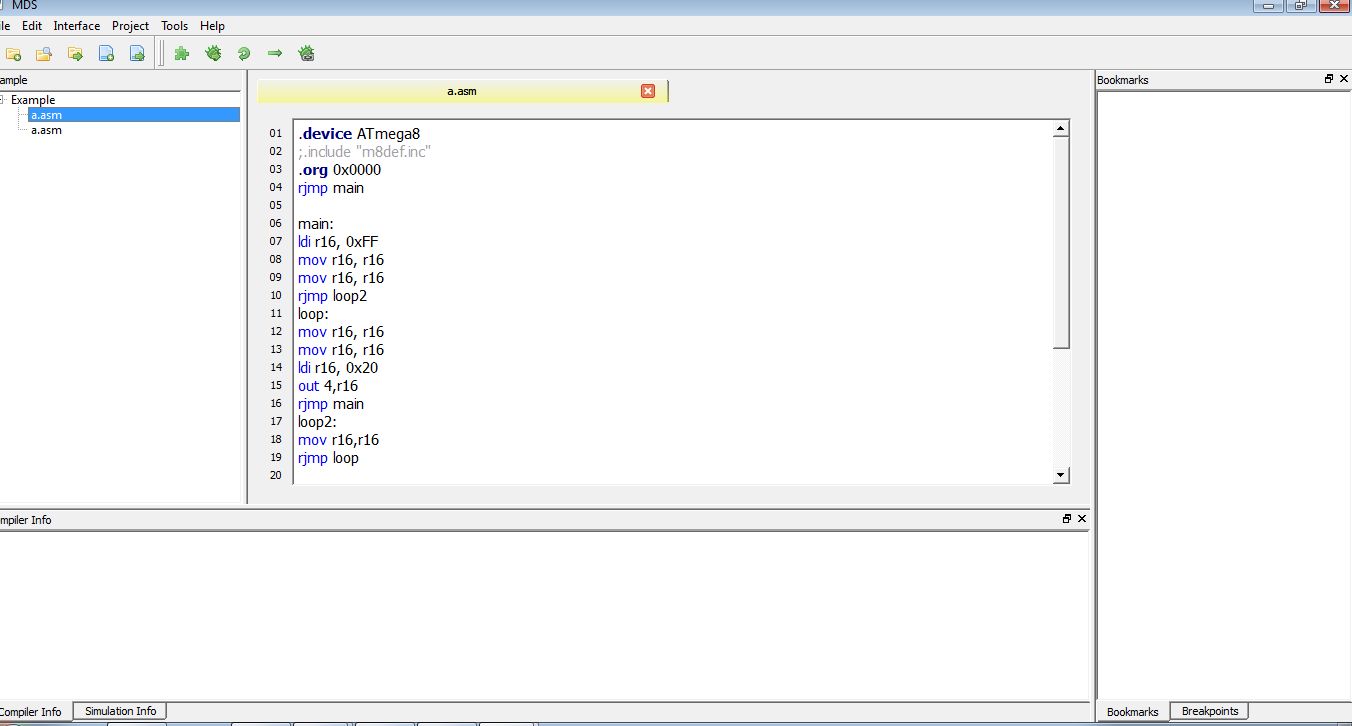
\includegraphics [scale=0.3]{img/Demonstration_project.png}
                      \caption{Window layout concept}
               \end{figure}

                \subsection{Source code editor}
                \subsection{Top panel}
                        \begin{figure}{r}{0pt}
                                \centering
                                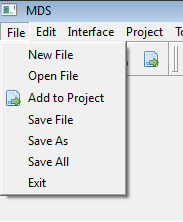
\includegraphics[width=110pt]{img/menu_file.png}
                                \caption{File selection}
                        \end{figure}

                        \begin{itemize}
                            \item New file: creates a new document to enter a new source file.
                            \item Open file: allows to open an existing source file.
                            \item Open recent: lists the 5 most recently used files.
                            \item Add to project:
                            \item Save file: saves the open document to the related file.
                            \item Save as: save the open document to a new file.
                            \item Save all: saves all currently open documents.
                            \item Exit: closes all open documents and closes MDS.
                        \end{itemize}

                        \begin{wrapfigure}{r}{0pt}
                                \centering
                                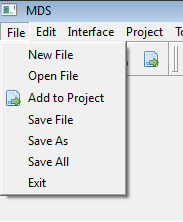
\includegraphics[width=110pt]{img/menu_file.png}
                                \caption{Edit selection}
                        \end{wrapfigure}

                        \begin{itemize}
                            \item Undo: will undo all edit actions on the open document in reverse order
                            \item Redo: will redo all undo actions
                            \item Cut: cuts all selected parts of the open doecument and puts it on the clipboard
                            \item Copy: copies all selected parts of the open document to the clipboard
                            \item Paste: pastes the text contents of the clipboard in the open document
                            \item Select: All selects all text in the open document
                            \item Find: find a to be given string through the open document
                            \item Replace: replace a given string in the open document by a new string
                        \end{itemize}

                        \begin{wrapfigure}{r}{0pt}
                                \centering
                                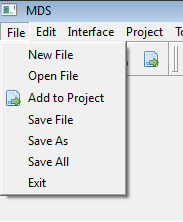
\includegraphics[width=110pt]{img/menu_file.png}
                                \caption{Project selection}
                        \end{wrapfigure}

                        \begin{itemize}
                            \item Undo: will undo all edit actions on the open document in reverse order
                            \item Redo: will redo all undo actions
                            \item Cut: cuts all selected parts of the open doecument and puts it on the clipboard
                            \item Copy: copies all selected parts of the open document to the clipboard
                            \item Paste: pastes the text contents of the clipboard in the open document
                            \item Select: All selects all text in the open document
                            \item Find: find a to be given string through the open document
                            \item Replace: replace a given string in the open document by a new string
                        \end{itemize}

                \subsection{Bottom panel}
                \subsection{Right panel}
                \subsection{Left panel}
                \subsection{Project configuration}
                In project configuration window, you can edit project and compiler settings.
                You can open project configuration window by right clicking to project name in the left panel. See the pictures below.
                    \begin{figure}
                        \centering{}
                        
\includegraphics [width=300pt]{img/mensi_obrazek.png}
                        \caption{Opening project configuration window from main screen}
                    \end{figure}
                This will open main configuration window with multiple tabs on the left side.
                        \begin{figure}
                            \centering{}
                            
\includegraphics [width=300pt]{img/mensi_obrazek.png}
                            \caption{Project window layout}
                        \end{figure}

                    \begin{itemize}
                        \item Undo: will undo all edit actions on the open document in reverse order
                        \item Redo: will redo all undo actions
                        \item Cut: cuts all selected parts of the open doecument and puts it on the clipboard
                        \item Copy: copies all selected parts of the open document to the clipboard
                        \item Paste: pastes the text contents of the clipboard in the open document
                        \item Select: All selects all text in the open document
                        \item Find: find a to be given string through the open document
                        \item Replace: replace a given string in the open document by a new string
                    \end{itemize}

                        \begin{figure}
                            \centering{}
                            
\includegraphics [width=300pt]{img/mensi_obrazek.png}
                            \caption{Project window layout}
                        \end{figure}

                    \begin{itemize}
                        \item Undo: will undo all edit actions on the open document in reverse order
                        \item Redo: will redo all undo actions
                        \item Cut: cuts all selected parts of the open doecument and puts it on the clipboard
                        \item Copy: copies all selected parts of the open document to the clipboard
                        \item Paste: pastes the text contents of the clipboard in the open document
                        \item Select: All selects all text in the open document
                        \item Find: find a to be given string through the open document
                        \item Replace: replace a given string in the open document by a new string
                    \end{itemize}

         \section{Other tools}
                \subsection{Code Completion list}
                The Code Completion List shows program symbols that contain
                the characters you are currently typing.
                        \begin{figure}
                            \centering{}
                            
\includegraphics [scale=0.3]{img/mensi_obrazek.png}
                            \caption{Code completion list}
                        \end{figure}

                \subsection{Parameter Information}
                    Parameter Information shows the names, amount of, and parameter types of a function or method. The
                    parameter in bold indicates the next parameter that is required as you are typing.
                    \begin{figure}
                        \centering{}
                        
\includegraphics [scale=0.3]{img/mensi_obrazek.png}
                        \caption{Parametr information list}
                    \end{figure}

                \subsection{DATA file convertor}
                    This tool alows you to convert selected data file to another. Mutual conversion can be made with
                    Hex, Bin, SRec, XilMem, XilVerilog and XilVhdl.
                    \begin{description}
                        \item[Section Input File] Here you can select desired input data file which is going to be converted
                        \item[Section Input Options] In this section, you define what type of input file is going to be converted
                        \item[Input file type] Available options - Hex, Bin, SRec, XilMem, XilVerilog and XilVhdl
                        \item[Bytes per record] Only if you want to convert XilMem file. Defines number of bytes per record
                        \item[OPCode size] Defines opcode size of selected data file. Available are 16 and 18
                        \item[Section Output File] Defines target
                        \item[Section Output Options] Here you can select desired output data file.
                        \item[Input file type] Available options - Hex, Bin, SRec, XilMem, XilVerilog and XilVhdl.
                        \item[Tab size]  Define number of inserted spaces when you press Tab.
                        \item[Short instructions] Here you can allow short instructions like LD, RETI or others
                    \end{description}

                    \begin{figure}
                        \centering{}
                        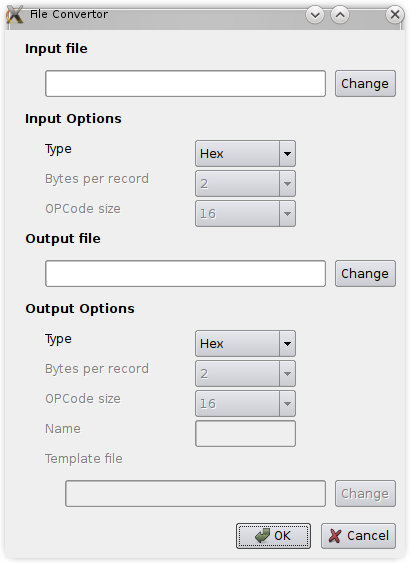
\includegraphics [scale=1]{img/DATA_convertor.png}
                        \caption{DATA file convertor}
                    \end{figure}

                \subsection{ASM translator}
                    With this tool, you can translate your previously written assembler code in different syntax.
                    You can sellect one of three choices - Xilinx, Mediatronix and OpenPicIde. Input code should be without
                    errors.
                    \begin{description}
                        \item[Section Input File] Here you can choose which file you want to translate into the MDS assembler
                        \item[Section ASM type] Input file syntax version. Translator needs to know input file syntax. Select one of three choices - Xilinx, Mediatronix and OpenPicIde
                        \item[Symbol] Case of symbols - UPPERCASE or LOWERCASE
                        \item[End of line] Indentation - Choose between Tabs or Spaces
                        \item[Directive] Case of Directives - UPPERCASE or LOWERCASE
                        \item[Indentation] Three choices - Tabs, Spaces and Keep (indentation unchanged)
                        \item[Instruction] Case of instructions - UPPERCASE or LOWERCASE
                        \item[Tab size]  Define number of inserted spaces when you press Tab.
                        \item[Short instructions] Here you can allow short instructions like LD, RETI or others
                    \end{description}

                    \begin{figure}
                        \centering{}
                        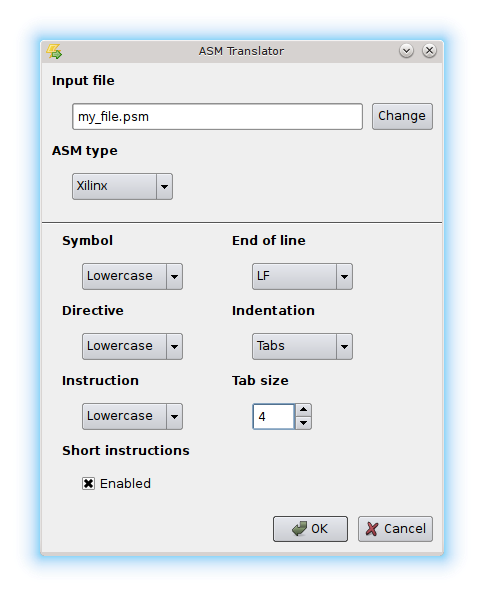
\includegraphics [scale=1]{img/ASM_translator.png}
                        \caption{ASM translator}
                    \end{figure}

                \subsection{Disassembler}
                    A disassembler is a tool that translates machine language into assembly language. The inverse
                    operation to that of an assembler.

                    \begin{description}
                        \item[Section File] Here you can choose which file you want to be disassembled
                        \item[Section Target] Architecture - Select processor architecture
                        \item[Family] select processor family of selected architecture
                        \item[Section Options] Indentation - Choose between Tabs or Spaces
                        \item[TabSize] Number of spaces in one tab
                        \item[Radix] Binary,Octal, Decima or Hexadecimal
                        \item[Linebreak] LF,CR or CRLF
                        \item[Case]  You can choose if you want disassemled file will be in upper or lower case
                        \item[Generate symbols] Select which symbols should be disassembled
                    \end{description}

                    \begin{figure}
                        \centering{}
                        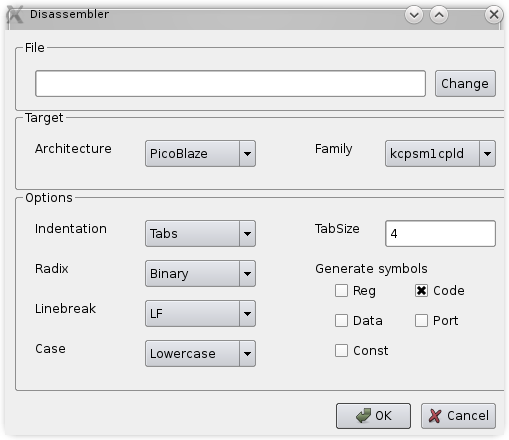
\includegraphics [scale=1]{img/disassembler_window.png}
                        \caption{Disassembler}
                    \end{figure}

                \subsection{Syntax Checking}
                    Syntax Checking validates the program syntax while you are typing
                    the code and provides real-time alerts to potential code violations
                    before compilation. This enhances productivity and greatly reduces
                    edit, compile, and correction cycles.
                    \begin{figure}
                        \centering{}
                        
\includegraphics [scale=0.3]{img/mensi_obrazek.png}
                        \caption{Syntax checking picture}
                    \end{figure}

                \subsection{Instruction details}
                \subsection{Subprograms call monitor}
                \subsection{ASCII chart}
                \subsection{PicoBlaze Instruction Table}
                \subsection{Symbol viewer}
                \subsection{Stopwatch}

                \subsection{Hexadecimal editors }
                \subsection{Interrupt monitor}

                \subsection{Number base converter}
                This tool is very usefull, when you want to find out the representation of given number in other
                number bases.

                        \begin{wrapfigure}{r}{0pt}
                                \centering
                                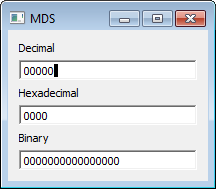
\includegraphics[width=110pt]{img/convertor.png}
                                \caption{Convertor}
                        \end{wrapfigure}

                \subsection{8-segment editor}
                With this tool you can easily determine what
                value you have to set on a port to display a digit
                on a numerical LED display. In the left part of
                the dialog window, you can find numerical val
                ues corresponding to the digit displayed in the
                middle part. These values are represented for
                both common cathode and anode and in three
                numerical bases, hexadecimal, decimal and oc
                tal. Buttons on left side from entry boxes copies
                value from adjacent entry box into clipboard.
                In the right part of the window you can set what port pin is connected to
                what LED segment.
                        \begin{wrapfigure}{r}{0pt}
                            \centering{}
                            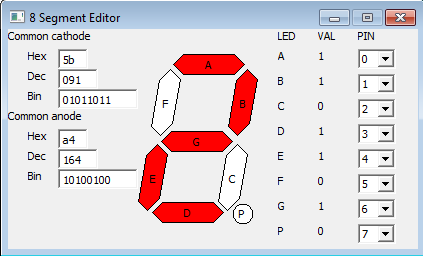
\includegraphics[width=110pt]{img/8segment.png}
                            \caption{8-segment editor}
                        \end{wrapfigure}


\chapter{MCU simulator}
  	\section{Short introduction}
        The MCU simulator is a tool designed to mimics behavior of a real MCU as
        much as possible. But it can have certain limitations, the most expectable
        limitation is of course the speed of simulation. This simulator is very slow,
        but ofers some extra features.
        \section{Modes of simulation}
        There are 4 modes of simulation:
            \begin{itemize}
                \item STEP: Execute exactly one intruction, no matter how many machine
                        cycles it will take. This does not apply for macro-instruction,
                        in that case each instruction of the macro is executed separately.
                \item STEP OVER: Execute as many instructions as possible until simulator
                cursor changes its location from one line of source code to another.
                \item ANIMATE: Do the same as step, but in a loop, one after another until
                stopped by a waring condition or user request.
                \item RUN: This is generally the same as animate, but much faster, because
                GUI is not updated so often as in the animate mode.
                \item STEP BACK: Take back the last performed step. There is limited number
                of step which can be taken back.
            \end{itemize}

\chapter{Built-in Macro assembler}
In this chapter, we will be concerned with build-in macro assembler.
With syntax of its statements, directives and PicoBlaze assembler instructions.
It is assumed, that the reader is familiar with general concepts of assembly
language programming and PicoBlaze architecture.\\\\
MDS has the most advanced macro assembler on the market. Its suports a lot of various
types of macros and advanced directives, like for example REPT and WHILE, which can create for and while loops or  macros with unlimited number of
input parameters.\\
Then each list element is beeing parsed and splitted into an address reference, a command and an argument list.
After them all directives are beeing filtered out and all commands and their arguments are beeing checked for validity.\\
\textbf{Important changes}\\
You need to tell compiler, that you are using constants by adding \# before second operand.

                \begin{code}[h!]
                        {\color{highlight_comment}\verb'; Example of instructions operating with constants'}\\
                        {\color{highlight_instruction}\verb'LOAD'}\verb'    '{\color{highlight_symbol}\verb's0,'}{\color{highlight_bin}\verb'#0b100111'}\verb'       '{\color{highlight_comment}\verb'; compiler now know, that this number is constant'}\\
                        {\color{highlight_instruction}\verb'LOAD'}\verb'    '{\color{highlight_symbol}\verb's0,'}{\color{highlight_bin}\verb'0b100'}\verb'       '{\color{highlight_comment}\verb'; and this compiler takes as an adrress'}\\
                        % Caption
                \end{code}

%%%%%%%%%%%%%%%%%%%%%%%%%%%%%%%%%%%%%%%%%%%%%%%%%%%%%%%%%%%%%%%%%%%%%%%%%%%
 	\section{Statements}
        Source code files for this assembler must be text files where lines are formed like these:\\
		\\ {
                \texttt{}
                \begin{tabular}[h!]{llll}
                        \verb'[' { \color{highlight_label} label: } \verb']' &
                        \verb'[' { \color{highlight_instruction} instruction } &
                        \verb'[' { \color{highlight_symbol} operand } \verb'[' , { \color{highlight_symbol} operand } \verb'[' , { \color{highlight_symbol} operand } \verb']' \verb']' \verb']' &
                        \verb'[' { \color{highlight_comment} ;comment } \verb']' \\

                        \verb'[' { \color{highlight_label} label: } \verb']' &
                        { \color{highlight_directive} directive } &
                        \verb'[' { \color{highlight_symbol} argument } \verb']' &
                        \verb'[' { \color{highlight_comment} ;comment } \verb']' \\

                        { \color{highlight_constant} symbol } &
                        { \color{highlight_directive} directive } &
                        { \color{highlight_symbol} argument } &
                        \verb'[' { \color{highlight_comment} ;comment } \verb']' \\

                        { \color{highlight_directive} directive } &
                        { \color{highlight_constant} symbol,argument } &
                         \verb'[' { \color{highlight_comment} ;comment } \verb']' \\
                \end{tabular}
                    }
                \bigskip
        Everything in square brackets is optional. Compilation does not go be-
        yond line containing "end" directive, so after that directive the code do not
        have to be syntactically valid. Empty lines are allowed as well as line contain-
        ing only comment or label. Statements can be separated by spaces, NBSP
        characters and tabs. Statements are case insensitive and their length is not
        limited, overall line length is also not limited.

    	\section{Symbols}
        Symbol names for numbers, macros or addresses defined by user in the code using
        appropriate directive. Like with ``\texttt{equ}'' directive you can define a new
        symbol and assign a value to it right away. Symbols may consist of upper and lower
        case letter, digits and underscore character (``\_''), their length is not limited,
        they are case insensitive and they can be the same as language keywords. Be aware of
        that there cannot coexists two or more symbols in the same memory segment which differs
        only by letter casing, in other words symbols ``\texttt{abc}'' and ``\texttt{ABC}''
        are completely the same thing.
                \begin{code}[h!]
                        {\color{highlight_comment}\verb'; Example of symbol definition'}\\
                        {\color{highlight_constant}\verb'First_symb'}\verb'    '{\color{highlight_directive}\verb'EQU'}\verb' '{\color{highlight_bin}\verb'0b100111'}\verb'   '{\color{highlight_comment}\verb'; Number in binary'}\\
                        {\color{highlight_constant}\verb'Second_symb'}\verb'   '{\color{highlight_directive}\verb'SET'}\verb' '{\color{highlight_oct}\verb'47q'}\verb'       '{\color{highlight_comment}\verb'; Octal'}\\
                        {\color{highlight_constant}\verb'Third_symb'}\verb'    '{\color{highlight_directive}\verb'REG'}\verb' '{\color{highlight_dec}\verb'39d'}\verb'       '{\color{highlight_comment}\verb'; Decimal'}\\
                        {\color{highlight_constant}\verb'Fourth_symb'}\verb'   '{\color{highlight_directive}\verb'DATA'}\verb' '{\color{highlight_hex}\verb'27h'}\verb'       '{\color{highlight_comment}\verb'; Hexadecimal'}\\
                        {\color{highlight_constant}\verb'Fifth_symb'}\verb'    '{\color{highlight_directive}\verb'CODE'}\verb' '{\color{highlight_hex}\verb'27h'}\verb'       '{\color{highlight_comment}\verb'; Hexadecimal'}\\
                        % Caption
                        \caption{An example of symbol definitons}
                \end{code}
        As you can see in Code 1 example, some unknown directives are used for symbol definition. Next chapter describes all directives, as well
        as constants syntax and expresions priority.

	\section{Constants}
        MDS supports both prefix and sufix definition.
                \begin{code}[h!]
                            {\color{highlight_comment}\verb'; Example of constants syntax'}\\
                            {\color{highlight_constant}\verb'10'}\verb' '\verb'   '{\color{highlight_comment}\verb'; Decimal'}\\
                            {\color{highlight_constant}\verb'10D'}\verb' '\verb'   '{\color{highlight_comment}\verb'; Decimal'}\\
                            {\color{highlight_constant}\verb'0xFE'}\verb' '\verb'   '{\color{highlight_comment}\verb'; Hexadecimal'}\\
                            {\color{highlight_constant}\verb'FEh'}\verb' '\verb'   '{\color{highlight_comment}\verb'; Hexadecimal'}\\
                            {\color{highlight_constant}\verb'O52'}\verb' '\verb'   '{\color{highlight_comment}\verb'; Octal'}\\
                            {\color{highlight_constant}\verb'52q'}\verb' '\verb'   '{\color{highlight_comment}\verb'; Octal'}\\
                            {\color{highlight_constant}\verb'01011110b'}\verb' '\verb'   '{\color{highlight_comment}\verb'; Binary'}\\
                            {\color{highlight_constant}\verb'0b00100001'}\verb' '\verb'   '{\color{highlight_comment}\verb'; Binary'}\\
                            {\color{highlight_constant}\verb'0b01'}\verb' '\verb'   '{\color{highlight_comment}\verb'; Binary, considers left side of byte zeroes'}\\
                            {\color{highlight_constant}\verb'01b'}\verb' '\verb'   '{\color{highlight_comment}\verb'; Binary, considers right side of byte zeroes'}\\
                            '\\\\s' ; Character
                            '\\\\n' ; Character
%             	            {\color{highlight_constant}\verb'\'\s\''}\verb' '\verb'   '{\color{highlight_comment}\verb'; Character'}\\
%             	            {\color{highlight_constant}\verb'\'\n\''}\verb' '\verb'   '{\color{highlight_comment}\verb'; Character'}\\
                                    % Caption

                    \caption{Syntax of various constant bases}
                \end{code}
                When you want to say to compiler, that you are using constant, you must add "\#" before.


        \section{Expressions}
        Arithmetical expressions are evaluated at compilation time and replaced by assembler
        with constant corresponding the their resulting value. Expressions comprises of arithmetical operators,
        constants, symbols and another expressions. An example of such expression might be
                \begin{itemize}
                    \item  \texttt{2+1}
                    \item  \texttt{(2 + 4) - ABC}
                    \item  \texttt{A \&\& B)} (
                    \item  \texttt{X XOR 0FF00H}
                    \item  \texttt{X * Y + X \% Y}
                \end{itemize}

        When multiple operators occur in an expression, the expression is evaluated in a specific order depending upon the operators in the expression.
        All LOGICAL operators have priorities lower than arithmetic and relational operators. Therefore, if an expression involving arithmetic, relational
        and logical operators, the arithmetic operators are evaluated first, followed by the relational operators, followed by the logical operators.
        The following table shows the priority of all the operators used in expressions.
		\begin{table}[h!]
			\mysmallfont{}
			\centering{}
			\begin{tabular}{|l|l|l|l|}
				\hline
                        Priority       &          Operator      & Description                   & Example               \\\hline

                        1              &          +           & unary plus sign              & +12                  \\\hline
                        1              &          -           & unary minus sign             & -5                   \\\hline
                        2              &           \verb'~'         & bitwise NOT		 	& \verb'~'0a55ah		\\\hline
                        2              &           !         & logical NOT		        & !0a55ah		\\\hline
                        3              &           *		& unsigned multiplication	& 11 * 12		\\\hline
                        3              &           /		& unsigned divisiono		& 11 / 12		\\\hline
                        3              &           \%		& unsigned remainder		& 13 \% 11		\\\hline
                        4              &           +		& unsigned addition	        & 3 + 5			\\\hline
                        4              &           -		& unsigned substraction		& 20 - 4		\\\hline
                        5              &           <<		& binary shift left		& 21 << 4		\\\hline
                        5              &           >>		& binary shift right		& 32 >> 2		\\\hline
                        6              &           <          & less than                    & 11 < 12              \\\hline
                        6              &           <=         & less or equal than           & 11 <= 11             \\\hline
                        6              &            >         & greater than                 & 12 > 11              \\\hline
                        6              &           >=         & greater or equal than        & 12 >= 11             \\\hline
                        7              &           ==         & equal to                     & 11 == 11             \\\hline
                        7              &           !=         & not equal to                 &  A != B              \\\hline
                        8              &           \&         & bitwise and                  & 48 \& 16              \\\hline
                        8              &           \verb'|'         & bitwise or                   & 370q \verb'|' 7             \\\hline
                        9              &           \&\&       & logical and                  & 48 \&\& 16           \\\hline
                        9              &           ||         & logical or                   & 370q || 7            \\\hline
                        9              &           \verb'^'		& exclusive or			& 00fh \verb'^' 005h		\\\hline
			\end{tabular}
			\caption{Expression operators priority}
		\end{table}
        A priority of 1 is the highest priority a priority of 9 is the lowest priority.
        When operators with different priority levels appear in an expression, operations are performed
        according to priorities. When operators of the same priority appear in an expression, operations are performed from left to right within
        the expression.

                \section{Predefined Symbols}
        There are symbols which are defined by default by assembler. The aim is to
        make it a little easier to write code in assembly language for Picoblaze,
        because user do not have to define all these symbols in his or her code.
                \begin{table}[h!]
                        \centering{}
                        \mysmallfont{}
                        \caption{Code addresses}
                        \begin{tabular}{|ll|}
                                \hline
                            \textbf{Symbol} & \textbf{Value} \\
                                \hline
                                s0      & 000h \\\hline
                                s1      & 001h  \\\hline
                               s2      & 002h \\\hline
                               s3      & 003h  \\\hline
                               s4      & 004h \\\hline
                               s5      & 005h  \\\hline
                               s6      & 006h \\\hline
                               s7      & 007h  \\\hline
                               s8      & 008h \\\hline
                               s9      & 009h  \\\hline
                               sA      & 00Ah \\\hline
                               sB      & 00Bh  \\\hline
                               sC      & 00Ch \\\hline
                               sD      & 00Dh  \\\hline
                               sE      & 00Eh \\\hline
                               sF      & 00Fh  \\\hline
                                \hline
                        \end{tabular}
                \end{table}


        \section{Assembler directives}
        Assembly directives are instructions
        that are executed by an assembler at assembly time,
        not by a CPU at run time. They can make the assembly of the program
        dependent on parameters input by a programmer, so that one program can be
        assembled different way, perhaps for different applications. They also
        can be used to manipulate presentation of a program to make it easier to read and maintain\\
        The specified format for most of the directives is:
		 \\
                 \\ {
                \texttt{}
                \begin{tabular}[h!]{llll}
                { \color{highlight_symbol} <symbol> }  &
                    { \color{highlight_directive} <directive> } &
                    { \color{highlight_constant} <expresion> } & { \color{highlight_comment} ; Directive syntax }\\
                \end{tabular}
      		 }
                 \\
        This syntax is valid for directives EQU, SET, REG, DATA, CODE, PORT, DEFINE.
        MDS also supports some other directives, with diferent syntax format, which is:
         \\      {
                \texttt{}
                \begin{tabular}[h!]{llll}
                        { \color{highlight_directive} <directive> } &
                        { \color{highlight_constant}\verb`<symbol>,<expresion>`  } & { \color{highlight_comment} ; Directive syntax }\\
                \end{tabular}
      		 }
           \\
        Those directives are CONSTANT, VARIABLE, ADRESS and NAMEREG. There are some other usefull directives like REPT or WHILE. See description below.

                \subsection{INCLUDE}
                \textbf{SYNTAX:}\\
                \\ {
                    \texttt{}
                    \begin{tabular}[h!]{llll}
                        { \color{highlight_directive} INCLUDE } & \verb`    ` &{ \color{highlight_symbol}\verb`"< file name >"`  }\\
                    \end{tabular}
                    }\\
                    \\
                \textbf{DESCRIPTION:}\\
                Compiler basicaly copies content of included file to line, where the directive is used. Include files can include other files.\\
                \textbf{EXAMPLE:}\\
                    \begin{code}[h!]
                        {\color{highlight_directive}\verb'INCLUDE'} \verb'    ' {\color{highlight_symbol}\verb' "LCD_characters"'}\\
                        {\color{highlight_directive}\verb'INCLUDE'} \verb'    ' {\color{highlight_symbol}\verb' "LCD_print_routine"'}\\
                        \verb'    '{\color{highlight_comment}\verb' ; this will replace includes with content of "LCD_characters" and "LCD_print_routine"'}\\
                        \caption{INCLUDE directive}
                    \end{code}

                \subsection{EQU}
                \textbf{SYNTAX:}\\
                        \\ {
                            \texttt{}
                            \begin{tabular}[h!]{llll}
                                    { \color{highlight_symbol} <symbol> }  &
                                    { \color{highlight_directive} EQU } &
                                    { \color{highlight_constant} <expresion> } & { \color{highlight_comment}  }\\
                            \end{tabular}
                        }\\
                        \\
                \textbf{DESCRIPTION:}\\
                The directive EQU stands for "equals". It allows you to give a numerical value to a symbol. This symbol cannot be redefined.
                \\
                \textbf{EXAMPLE:}\\
                        \begin{code}[h!]
                                {\color{highlight_constant}\verb'First_symb'}\verb'    '{\color{highlight_directive}\verb'EQU'}\verb' '{\color{highlight_bin}\verb'0b10011100'}\verb'   '{\color{highlight_comment}\verb'; Number in binary'}\\
                                {\color{highlight_constant}\verb'Second_symb'}\verb'   '{\color{highlight_directive}\verb'EQU'}\verb' '{\color{highlight_oct}\verb'47'}\verb'       '{\color{highlight_comment}\verb'; Decimal'}\\
                                {\color{highlight_constant}\verb'Third_symb'}\verb'    '{\color{highlight_directive}\verb'EQU'}\verb' '{\color{highlight_dec}\verb'0x39'}\verb'       '{\color{highlight_comment}\verb'; Hexadecimal'}\\
                                {\color{highlight_constant}\verb'Fourth_symb'}\verb'   '{\color{highlight_directive}\verb'EQU'}\verb' '{\color{highlight_dec}\verb'(A -4)+ 18 / B)'}\verb'       '{\color{highlight_comment}\verb'; Expresion'}\\
                                {\color{highlight_constant}\verb'Fifth_symb'}\verb'    '{\color{highlight_directive}\verb'EQU'}\verb' '{\color{highlight_dec}\verb'0x09 << 2'}\verb'       '{\color{highlight_comment}\verb'; Expresion'}\\
                        \caption{Using EQU directive}
                    \end{code}

            In this example, the assembler would always replace {\color{highlight_symbol}\verb'First_symb'} with 0x9C,
            {\color{highlight_symbol}\verb'Second_symb'} with 0x2F and {\color{highlight_symbol}\verb'Third_symb'} with 0x39.

                \subsection{CONSTANT}
                \textbf{SYNTAX:}\\
                    \\ {
                        \texttt{}
                        \begin{tabular}[h!]{llll}
                                { \color{highlight_directive} CONSTANT } &
                                { \color{highlight_symbol} <symbol> }  &
                                \verb',' &
                                { \color{highlight_constant} <expresion> }\\
                        \end{tabular}
                    }\\
                    \\
                \textbf{DESCRIPTION:}\\
                The directive CONSTANT allows you to give a numerical value to a symbol. It is same like EQU, but with diferent syntax. Cannot be redefined.\\

                \textbf{EXAMPLE:}\\
                    \begin{code}[h!]
                        %\mysmallfont{}
                                {\color{highlight_directive}\verb'CONSTANT'}\verb'    '{\color{highlight_symbol}\verb'First_symb'}\verb','{\color{highlight_constant}\verb'0b10011100'}\verb'   '{\color{highlight_comment}\verb'; Number in binary'}\\
                                {\color{highlight_directive}\verb'CONSTANT'}\verb'    '{\color{highlight_symbol}\verb'Second_symb'}\verb','{\color{highlight_constant}\verb'47'}\verb'       '{\color{highlight_comment}\verb'; Decimal'}\\
                                {\color{highlight_directive}\verb'CONSTANT'}\verb'    '{\color{highlight_symbol}\verb'Third_symb'}\verb','{\color{highlight_constant}\verb'0x39'}\verb'       '{\color{highlight_comment}\verb'; Hexadecimal'}\\
                        \caption{Using CONSTANT directive}
                    \end{code}

                In this example, the assembler would always replace {\color{highlight_symbol}\verb'First_symb'} with 0x9C,
                {\color{highlight_symbol}\verb'Second_symb'} with 0x2F and {\color{highlight_symbol}\verb'Third_symb'} with 0x39 etc.

            \subsection{SET}
            \textbf{SYNTAX:}\\
                    \\ {
                            \texttt{}
                            \begin{tabular}[h!]{llll}
                            { \color{highlight_symbol} <symbol> }  &
                            { \color{highlight_directive} SET } &
                            { \color{highlight_constant} <expresion> } & { \color{highlight_comment}  }\\
                            \end{tabular}
                    }
                    \\

            \textbf{DESCRIPTION:}\\
            Directive SET is quite similar to EQU, but symbols defined with the SET(and Variable) directive can be redefined with another value in your source
            code, but those defined with EQU cannot.\\

            \textbf{EXAMPLE:}\\
                \begin{code}[h!]
                \mysmallfont{}
                            {\color{highlight_constant}\verb'First_symb'}\verb'    '{\color{highlight_directive}\verb'SET'}\verb' '{\color{highlight_bin}\verb'0b10011100'}\verb'   '{\color{highlight_comment}\verb'; Number in binary'}\\
                            {\color{highlight_constant}\verb'Second_symb'}\verb'   '{\color{highlight_directive}\verb'SET'}\verb' '{\color{highlight_oct}\verb'47'}\verb'       '{\color{highlight_comment}\verb'; Decimal'}\\
                            {\color{highlight_constant}\verb'Third_symb'}\verb'    '{\color{highlight_directive}\verb'SET'}\verb' '{\color{highlight_dec}\verb'0x39'}\verb'       '{\color{highlight_comment}\verb'; Hexadecimal'}\\
                            {\color{highlight_constant}\verb'Fourth_symb'}\verb'   '{\color{highlight_directive}\verb'SET'}\verb' '{\color{highlight_dec}\verb'(A -4)+ 18 / B)'}\verb'       '{\color{highlight_comment}\verb'; Expresion'}\\
                            {\color{highlight_constant}\verb'Fifth_symb'}\verb'    '{\color{highlight_directive}\verb'SET'}\verb' '{\color{highlight_dec}\verb'0x09 << 2'}\verb'       '{\color{highlight_comment}\verb'; Expresion'}\\
                \caption{Using SET directive}
                \end{code}

            In this example, the assembler would always replace {\color{highlight_symbol}\verb'First_symb'} with 0x9C,
            {\color{highlight_symbol}\verb'Second_symb'} with 0x2F and {\color{highlight_symbol}\verb'Third_symb'} with 0x39 etc.

            \subsection{VARIABLE}
            \textbf{SYNTAX:}\\
                \\ {
                    \texttt{}
                    \begin{tabular}[h!]{llll}
                            { \color{highlight_directive} VARIABLE } &
                            { \color{highlight_symbol} <symbol> }  &
                            \verb',' &
                            { \color{highlight_constant} <expresion> }\\
                    \end{tabular}
                }\\
                \\
            \textbf{DESCRIPTION:}\\
            Directive VARIABLE is similar to SET, but with diferent syntax. Symbols defined with VARIABLE can be redefined with another value in your source
            code, but those defined with EQU cannot.

            \textbf{EXAMPLE:}\\
                    \begin{code}[h!]
                            %\mysmallfont{}
                                    {\color{highlight_directive}\verb'VARIABLE'}\verb'    '{\color{highlight_symbol}\verb'First_symb'}\verb','{\color{highlight_constant}\verb'0b10011100'}\verb'   '{\color{highlight_comment}\verb'; Number in binary'}\\
                                    {\color{highlight_directive}\verb'VARIABLE'}\verb'    '{\color{highlight_symbol}\verb'Second_symb'}\verb','{\color{highlight_constant}\verb'47'}\verb'       '{\color{highlight_comment}\verb'; Decimal'}\\
                                    {\color{highlight_directive}\verb'VARIABLE'}\verb'    '{\color{highlight_symbol}\verb'Third_symb'}\verb','{\color{highlight_constant}\verb'0x39'}\verb'       '{\color{highlight_comment}\verb'; Hexadecimal'}\\
                            \caption{Using CONSTANT directive}
                    \end{code}

            In this example, the assembler would always replace {\color{highlight_symbol}\verb'First_symb'} with 0x9C,
            {\color{highlight_symbol}\verb'Second_symb'} with 0x2F and {\color{highlight_symbol}\verb'Third_symb'} with 0x39.

                \subsection{REG}
                \textbf{SYNTAX:}\\
                                \\ {
                                        \texttt{}
                                        \begin{tabular}[h!]{llll}
                                        { \color{highlight_symbol} <symbol> }  &
                                        { \color{highlight_directive} REG } &
                                        { \color{highlight_constant} <expresion> } & { \color{highlight_comment} }\\
                                        \end{tabular}
                                }
                                \\

                \textbf{DESCRIPTION:}\\
                Symbols defined with the REG directive are by compiler considered as work registers.

                \textbf{EXAMPLE:}\\
                       \begin{code}[h!]
                \mysmallfont{}
                            {\color{highlight_constant}\verb'First_symb'}\verb'    '{\color{highlight_directive}\verb'REG'}\verb' '{\color{highlight_bin}\verb'0b10011100'}\verb'   '{\color{highlight_comment}\verb'; Number in binary'}\\
                            {\color{highlight_constant}\verb'Second_symb'}\verb'   '{\color{highlight_directive}\verb'REG'}\verb' '{\color{highlight_oct}\verb'47'}\verb'       '{\color{highlight_comment}\verb'; Decimal'}\\
                            {\color{highlight_constant}\verb'Third_symb'}\verb'    '{\color{highlight_directive}\verb'REG'}\verb' '{\color{highlight_dec}\verb'0x39'}\verb'       '{\color{highlight_comment}\verb'; Hexadecimal'}\\
                            {\color{highlight_constant}\verb'Fourth_symb'}\verb'   '{\color{highlight_directive}\verb'REG'}\verb' '{\color{highlight_dec}\verb'(A -4)+ 18 / B)'}\verb'       '{\color{highlight_comment}\verb'; Expresion'}\\
                            {\color{highlight_constant}\verb'Fifth_symb'}\verb'    '{\color{highlight_directive}\verb'REG'}\verb' '{\color{highlight_dec}\verb'0x09 << 2'}\verb'       '{\color{highlight_comment}\verb'; Expresion'}\\
              \caption{Using REG directive}
                \end{code}

            In this example, the assembler would always replace {\color{highlight_symbol}\verb'First_symb'} with 0x9C,
            {\color{highlight_symbol}\verb'Second_symb'} with 0x2F and {\color{highlight_symbol}\verb'Third_symb'} with 0x39 etc.

                \subsection{NAMEREG}
                \textbf{SYNTAX:}\\
                    \\ {
                        \texttt{}
                        \begin{tabular}[h!]{llll}
                                { \color{highlight_directive} NAMEREG } &
                                { \color{highlight_symbol} <symbol> }  &
                                \verb',' &
                                { \color{highlight_constant} <expresion> }\\
                        \end{tabular}
                    }\\
                    \\
                \textbf{DESCRIPTION:}\\
                Directive NAMEREG is similar to REG, but with diferent syntax. Symbols defined with NAMEREG can be redefined with another value in your source
                code.

                \textbf{EXAMPLE:}\\
                \begin{code}[h!]
                        %\mysmallfont{}
                                {\color{highlight_directive}\verb'NAMEREG'}\verb'    '{\color{highlight_symbol}\verb'First_symb'}\verb','{\color{highlight_constant}\verb'0b10011100'}\verb'   '{\color{highlight_comment}\verb'; Number in binary'}\\
                                {\color{highlight_directive}\verb'NAMEREG'}\verb'    '{\color{highlight_symbol}\verb'Second_symb'}\verb','{\color{highlight_constant}\verb'47'}\verb'       '{\color{highlight_comment}\verb'; Decimal'}\\
                                {\color{highlight_directive}\verb'NAMEREG'}\verb'    '{\color{highlight_symbol}\verb'Third_symb'}\verb','{\color{highlight_constant}\verb'0x39'}\verb'       '{\color{highlight_comment}\verb'; Hexadecimal'}\\
                        \caption{Using CONSTANT directive}
                    \end{code}

                In this example, the assembler would always replace {\color{highlight_symbol}\verb'First_symb'} with 0x9C,
                {\color{highlight_symbol}\verb'Second_symb'} with 0x2F and {\color{highlight_symbol}\verb'Third_symb'} with 0x39.



                \subsection{DATA}
                \textbf{SYNTAX:}\\
                                \\ {
                                        \texttt{}
                                        \begin{tabular}[h!]{llll}
                                        { \color{highlight_symbol} <symbol> }  &
                                        { \color{highlight_directive} DATA } &
                                        { \color{highlight_constant} <expresion> } & { \color{highlight_comment}  }\\
                                        \end{tabular}
                                }
                                \\
                \textbf{DESCRIPTION:}\\
               Symbols defined with the DATA directive are by compiler considered as data memory. It must be used only with instructions FETCH and STORE.

                \textbf{EXAMPLE:}\\
                \begin{code}[h!]
                            {\color{highlight_constant}\verb'First_symb'}\verb'    '{\color{highlight_directive}\verb'DATA'}\verb' '{\color{highlight_bin}\verb'0b10011100'}\verb'   '{\color{highlight_comment}\verb'; Number in binary'}\\
                            {\color{highlight_constant}\verb'Second_symb'}\verb'   '{\color{highlight_directive}\verb'DATA'}\verb' '{\color{highlight_oct}\verb'47'}\verb'       '{\color{highlight_comment}\verb'; Decimal'}\\
                            {\color{highlight_constant}\verb'Third_symb'}\verb'    '{\color{highlight_directive}\verb'DATA'}\verb' '{\color{highlight_dec}\verb'0x39'}\verb'       '{\color{highlight_comment}\verb'; Hexadecimal'}\\
                            {\color{highlight_constant}\verb'Fourth_symb'}\verb'   '{\color{highlight_directive}\verb'DATA'}\verb' '{\color{highlight_dec}\verb'(A -4)+ 18 / B)'}\verb'       '{\color{highlight_comment}\verb'; Expresion'}\\
                            {\color{highlight_constant}\verb'Fifth_symb'}\verb'    '{\color{highlight_directive}\verb'DATA'}\verb' '{\color{highlight_dec}\verb'0x09 << 2'}\verb'       '{\color{highlight_comment}\verb'; Expresion'}\\
              \caption{Using DATA directive}
                \end{code}

            In this example, the assembler would always replace {\color{highlight_symbol}\verb'First_symb'} with 0x9C,
            {\color{highlight_symbol}\verb'Second_symb'} with 0x2F and {\color{highlight_symbol}\verb'Third_symb'} with 0x39 etc.

                \subsection{CODE}
                \textbf{SYNTAX:}\\
                                \\ {
                                        \texttt{}
                                        \begin{tabular}[h!]{llll}
                                        { \color{highlight_symbol} <symbol> }  &
                                        { \color{highlight_directive} CODE } &
                                        { \color{highlight_constant} <expresion> } & { \color{highlight_comment}  }\\
                                        \end{tabular}
                                }
                                \\
                \textbf{DESCRIPTION:}\\
                Symbols defined with the CODE directive are by compiler considered as program memory.

                \textbf{EXAMPLE:}\\
                \begin{code}[h!]
                \mysmallfont{}
                            {\color{highlight_constant}\verb'First_symb'}\verb'    '{\color{highlight_directive}\verb'CODE'}\verb' '{\color{highlight_bin}\verb'0b10011100'}\verb'   '{\color{highlight_comment}\verb'; Number in binary'}\\
                            {\color{highlight_constant}\verb'Second_symb'}\verb'   '{\color{highlight_directive}\verb'CODE'}\verb' '{\color{highlight_oct}\verb'47'}\verb'       '{\color{highlight_comment}\verb'; Decimal'}\\
                            {\color{highlight_constant}\verb'Third_symb'}\verb'    '{\color{highlight_directive}\verb'CODE'}\verb' '{\color{highlight_dec}\verb'0x39'}\verb'       '{\color{highlight_comment}\verb'; Hexadecimal'}\\
                            {\color{highlight_constant}\verb'Fourth_symb'}\verb'   '{\color{highlight_directive}\verb'CODE'}\verb' '{\color{highlight_dec}\verb'(A -4)+ 18 / B)'}\verb'       '{\color{highlight_comment}\verb'; Expresion'}\\
                            {\color{highlight_constant}\verb'Fifth_symb'}\verb'    '{\color{highlight_directive}\verb'CODE'}\verb' '{\color{highlight_dec}\verb'0x09 << 2'}\verb'       '{\color{highlight_comment}\verb'; Expresion'}\\
                            \caption{Using CODE directive}
                \end{code}

            In this example, the assembler would always replace {\color{highlight_symbol}\verb'First_symb'} with 0x9C,
            {\color{highlight_symbol}\verb'Second_symb'} with 0x2F and {\color{highlight_symbol}\verb'Third_symb'} with 0x39 etc.

                \subsection{PORT}
                \textbf{SYNTAX:}\\
                                \\ {
                                        \texttt{}
                                        \begin{tabular}[h!]{llll}
                                        { \color{highlight_symbol} <symbol> }  &
                                        { \color{highlight_directive} PORT } &
                                        { \color{highlight_constant} <expresion> } & { \color{highlight_comment}  }\\
                                        \end{tabular}
                                }
                                \\
                \textbf{DESCRIPTION:}\\
                Symbol defined with this directive is considered to be PORT\_ID identificator.

                \textbf{EXAMPLE:}\\
                \begin{code}[h!]
                \mysmallfont{}
                            {\color{highlight_constant}\verb'First_symb'}\verb'    '{\color{highlight_directive}\verb'PORT'}\verb' '{\color{highlight_bin}\verb'0b10011100'}\verb'   '{\color{highlight_comment}\verb'; Number in binary'}\\
                            {\color{highlight_constant}\verb'Second_symb'}\verb'   '{\color{highlight_directive}\verb'PORT'}\verb' '{\color{highlight_oct}\verb'47'}\verb'       '{\color{highlight_comment}\verb'; Decimal'}\\
                            {\color{highlight_constant}\verb'Third_symb'}\verb'    '{\color{highlight_directive}\verb'PORT'}\verb' '{\color{highlight_dec}\verb'0x39'}\verb'       '{\color{highlight_comment}\verb'; Hexadecimal'}\\
                            {\color{highlight_constant}\verb'Fourth_symb'}\verb'   '{\color{highlight_directive}\verb'PORT'}\verb' '{\color{highlight_dec}\verb'(A -4)+ 18 / B)'}\verb'       '{\color{highlight_comment}\verb'; Expresion'}\\
                            {\color{highlight_constant}\verb'Fifth_symb'}\verb'    '{\color{highlight_directive}\verb'PORT'}\verb' '{\color{highlight_dec}\verb'0x09 << 2'}\verb'       '{\color{highlight_comment}\verb'; Expresion'}\\
              \caption{Using PORT directive}
                \end{code}

            In this example, the assembler would always replace {\color{highlight_symbol}\verb'First_symb'} with 0x9C,
            {\color{highlight_symbol}\verb'Second_symb'} with 0x2F and {\color{highlight_symbol}\verb'Third_symb'} with 0x39 etc.


                \subsection{AUTOREG}
                \textbf{SYNTAX:}\\
                        \\ {
                                \texttt{}
                                \begin{tabular}[h!]{llll}
                                { \color{highlight_symbol} <symbol> }  &
                                { \color{highlight_directive} AUTOREG }
                                { \color{highlight_constant} [AT E] } & { \color{highlight_comment} ; Optional attribute can define
                                                                                                    counter starting adress }\\
                                \end{tabular}
                        }
                        \\

                \textbf{DESCRIPTION:}\\
                This directive saves time. You can use it, when you dont care which work register will be used. It will automatically assign a register
                at adress 0x00, which is incremented with every other AUTOREG directive. Optionaly, you can change starting address counter by adding a parameter
                after AUTOREG directive. You can check assigned registers in codelisting (file .lst) and symbol table (file .sym).

                \textbf{EXAMPLE:}\\
                        \begin{code}[h!]
                        \mysmallfont{}
                                {\color{highlight_symbol}\verb'First_symb'}\verb'   '{\color{highlight_directive}\verb'AUTOREG'}\verb'   '
                                {\color{highlight_comment}\verb'; Automaticaly assigned, register at adress 0x00'}\\
                                {\color{highlight_symbol}\verb'Second_symb'}\verb'   '{\color{highlight_directive}\verb'AUTOREG'}\verb'   '
                                \verb'  '{\color{highlight_comment}\verb'; Adress incremented, register at adress 0x01 '}\\
                                {\color{highlight_symbol}\verb'Third_symb'}\verb'   '{\color{highlight_directive}\verb'AUTOREG'}\verb'   '
                                \verb'  '{\color{highlight_comment}\verb'; Adress incremented, register at adress 0x02 '}\\
                                {\color{highlight_comment}\verb'; Now with optional parameter changing counting adress '}\\
                                {\color{highlight_symbol}\verb'Fourth_symb'}\verb'   '{\color{highlight_directive}\verb'AUTOREG'}\verb'   '
                                {\color{highlight_symbol}\verb'AT 10h'}\verb'  '{\color{highlight_comment}\verb'; Registers are now defined from adress 0x10 '}
                                {\color{highlight_symbol}\verb'Fifth_symb'}\verb'   '{\color{highlight_directive}\verb'AUTOREG'}\verb'   '
                                {\color{highlight_comment}\verb'; Now register at adress 0x11'}\\
                        \caption{Using AUTOREG directive}
                    \end{code}

                \subsection{AUTOSPR}
                \textbf{SYNTAX:}\\
                            \\ {
                                    \texttt{}
                                    \begin{tabular}[h!]{llll}
                                    { \color{highlight_symbol} <symbol> }  &
                                    { \color{highlight_directive} AUTOSPR }
                                    { \color{highlight_constant} [AT E] } & { \color{highlight_comment} ; Optional attribute can define
                                                                                                        counter starting adress }\\
                                    { \color{highlight_constant} length } & { \color{highlight_comment} ; Optional attribute can define
                                                                                                        counter starting adress }\\
                                    \end{tabular}
                            }
                            \\
            \textbf{DESCRIPTION:}\\
            Must be used only with instructions FETCH and STORE. It will automatically assign an
            adress 0x00, which is incremented with every other AUTOSPR directive. Optionaly, you can change starting address counter by adding a parameter
            after AUTOSPR directive. You can check assigned memory in codelisting file(.lst) and symbol table file(.sym).

            \textbf{EXAMPLE:}\\
                    \begin{code}[h!]
                    \mysmallfont{}
                            {\color{highlight_symbol}\verb'First_symb'}\verb'   '{\color{highlight_directive}\verb'AUTOSPR'}\verb'   '
                            {\color{highlight_comment}\verb'; Automaticaly assigned, register at adress 0x00'}\\
                            {\color{highlight_symbol}\verb'Second_symb'}\verb'   '{\color{highlight_directive}\verb'AUTOSPR'}\verb'   '
                            \verb'  '{\color{highlight_comment}\verb'; Adress incremented, register at adress 0x01 '}\\
                            {\color{highlight_symbol}\verb'Third_symb'}\verb'   '{\color{highlight_directive}\verb'AUTOSPR'}\verb'   '
                            \verb'  '{\color{highlight_comment}\verb'; Adress incremented, register at adress 0x02 '}\\
                            {\color{highlight_comment}\verb'; Now with optional parameter changing counting adress '}\\
                            {\color{highlight_symbol}\verb'Fourth_symb'}\verb'   '{\color{highlight_directive}\verb'AUTOSPR'}\verb'   '
                            {\color{highlight_symbol}\verb'10h'}\verb'  '{\color{highlight_comment}\verb'; Registers are now defined from adress 0x10 '}
                            {\color{highlight_symbol}\verb'Fifth_symb'}\verb'   '{\color{highlight_directive}\verb'AUTOSPR'}\verb'   '
                            {\color{highlight_comment}\verb'; Now register at adress 0x11'}\\
                    \caption{Using AUTOREG directive}
                \end{code}
                
               \subsection{INITSPR}
                \textbf{SYNTAX:}\\
                            \\ {
                                    \texttt{}
                                    \begin{tabular}[h!]{llll}
                                    { \color{highlight_symbol} <symbol> }  &
                                    { \color{highlight_directive} AUTOSPR }
                                    { \color{highlight_constant} [AT E] } & { \color{highlight_comment} ; Optional attribute can define
                                                                                                        counter starting adress }\\
                                    \end{tabular}
                            }
                            \\
            \textbf{DESCRIPTION:}\\
            Another time saving directive. Must be used only with instructions FETCH and STORE. It will automatically assign an
            adress 0x00, which is incremented with every other AUTOSPR directive. Optionaly, you can change starting address counter by adding a parameter
            after AUTOSPR directive. You can check assigned memory in codelisting file(.lst) and symbol table file(.sym).

            \textbf{EXAMPLE:}\\
                    \begin{code}[h!]
                    \mysmallfont{}
                            {\color{highlight_symbol}\verb'First_symb'}\verb'   '{\color{highlight_directive}\verb'AUTOSPR'}\verb'   '
                            {\color{highlight_comment}\verb'; Automaticaly assigned, register at adress 0x00'}\\
                            {\color{highlight_symbol}\verb'Second_symb'}\verb'   '{\color{highlight_directive}\verb'AUTOSPR'}\verb'   '
                            \verb'  '{\color{highlight_comment}\verb'; Adress incremented, register at adress 0x01 '}\\
                            {\color{highlight_symbol}\verb'Third_symb'}\verb'   '{\color{highlight_directive}\verb'AUTOSPR'}\verb'   '
                            \verb'  '{\color{highlight_comment}\verb'; Adress incremented, register at adress 0x02 '}\\
                            {\color{highlight_comment}\verb'; Now with optional parameter changing counting adress '}\\
                            {\color{highlight_symbol}\verb'Fourth_symb'}\verb'   '{\color{highlight_directive}\verb'AUTOSPR'}\verb'   '
                            {\color{highlight_symbol}\verb'10h'}\verb'  '{\color{highlight_comment}\verb'; Registers are now defined from adress 0x10 '}
                            {\color{highlight_symbol}\verb'Fifth_symb'}\verb'   '{\color{highlight_directive}\verb'AUTOSPR'}\verb'   '
                            {\color{highlight_comment}\verb'; Now register at adress 0x11'}\\
                    \caption{Using AUTOREG directive}
                \end{code}

                \subsection{ORGSPR, MERGESPR}
                \textbf{SYNTAX:}\\
                \\ {
                        \texttt{}
                        \begin{tabular}[h!]{llll}
                                { \color{highlight_directive} ORGSPR } & \verb'         '
                                { \color{highlight_constant} <address> } & { \color{highlight_comment}  }\\
                        \end{tabular}
                    }\\
                \\ {
                        \texttt{}
                        \begin{tabular}[h!]{llll}
                                { \color{highlight_directive} MERGESPR } & \verb'         '
                                { \color{highlight_constant} <address>,<size> } & { \color{highlight_comment}  }\\
                        \end{tabular}
                    }\\
                \textbf{DESCRIPTION:}\\
                When the ORG or ADDRESS statement is encountered, the assembler calculates the value of the expression and changes the address counter.
                The MDS assembler maintains a location counter for each segment. The location counter contains the offset of the instruction or data
                being assembled and is incremented after each line by the number of bytes of data or code in that line.
                \textbf{EXAMPLE:}\\
                        \begin{code}[h!]
                                \verb'    '{\color{highlight_directive}\verb'ORG'}\verb'   '{\color{highlight_constant}\verb'0x3FF'}\verb'                  '{\color{highlight_comment}\verb'; Number'}\\
                                \verb'    '{\color{highlight_directive}\verb'ORG'}\verb'   '{\color{highlight_label}\verb'START:'}\verb'                    '{\color{highlight_comment}\verb'; Symbol'}\\
                                \verb'    '{\color{highlight_directive}\verb'ORG'}\verb'   '{\color{highlight_label}\verb'INTERRUPT'}\verb'                 '{\color{highlight_comment}\verb'; Symbol'}\\
                                \verb'    '{\color{highlight_directive}\verb'ORG'}\verb'   '{\color{highlight_constant}\verb'($ + 15) AND 0xFFEE'}\verb'    '{\color{highlight_comment}\verb'; Expresion'}\\
                        \caption{Using ORG directive}
                        \end{code}
                        \begin{code}[h!]
                                \verb'    '{\color{highlight_directive}\verb'ADDRESS'}\verb'   '{\color{highlight_constant}\verb'0x3FF'}\verb'                  '{\color{highlight_comment}\verb'; Number'}\\
                                \verb'    '{\color{highlight_directive}\verb'ADDRESS'}\verb'   '{\color{highlight_label}\verb'START:'}\verb'                    '{\color{highlight_comment}\verb'; Symbol'}\\
                                \verb'    '{\color{highlight_directive}\verb'ADDRESS'}\verb'   '{\color{highlight_label}\verb'INTERRUPT'}\verb'                 '{\color{highlight_comment}\verb'; Symbol'}\\
                                \verb'    '{\color{highlight_directive}\verb'ADDRESS'}\verb'   '{\color{highlight_constant}\verb'($ + 15) AND 0xFFEE'}\verb'    '{\color{highlight_comment}\verb'; Expresion'}\\
                        \caption{Using ADDRESS directive}
                        \end{code}
 
                
                \subsection{DEFINE}
                \textbf{SYNTAX:}\\
                \\ {
                        \texttt{}
                        \begin{tabular}[h!]{llll}
                                { \color{highlight_symbol} <symbol> }  &
                                { \color{highlight_directive} DEFINE } &
                                { \color{highlight_constant} <expresion> } & { \color{highlight_comment}  }\\
                        \end{tabular}
                    }\\
                    \\

                \textbf{DESCRIPTION:}\\
                You can define expresion using previously defined symbols. Value of this expresion is calculated every time the symbol is used.

                \textbf{EXAMPLE:}\\
                                \begin{code}[h!]
                                    {\color{highlight_symbol}\verb'A'}\verb'   '{\color{highlight_directive}\verb'EQU'}\verb' '
                                    {\color{highlight_oct}\verb'10'}\verb'       '{\color{highlight_comment}\verb'; First symbol'}\\
                                    {\color{highlight_symbol}\verb'B'}\verb'   '{\color{highlight_directive}\verb'SET'}\verb' '
                                    {\color{highlight_oct}\verb'5'}\verb'       '{\color{highlight_comment}\verb'; Second  symbol, redefinable'}\\
                                    {\color{highlight_symbol}\verb'C'}\verb'    '{\color{highlight_directive}\verb'DEFINE'}\verb' '
                                    {\color{highlight_constant}\verb'(A + B) * 2'}\verb'   '{\color{highlight_comment}\verb'; Defined expresion'}\\
                                    {\color{highlight_symbol}\verb'C = '}{\color{highlight_constant}\verb'30'}\\
                                    {\color{highlight_symbol}\verb'B'}\verb'   '{\color{highlight_directive}\verb'SET'}\verb' '
                                    {\color{highlight_oct}\verb'10'}\verb'       '{\color{highlight_comment}\verb'; B redefined'}\\
                                    {\color{highlight_symbol}\verb'C = '}{\color{highlight_constant}\verb'40'}\verb'   '{\color{highlight_comment}\verb'; C is now different'}\\\\
                                \caption{Example of DEFINE directive}
                                \end{code}

               \subsection{ADDRESS,ORG}
                \textbf{SYNTAX:}\\
                \\ {
                        \texttt{}
                        \begin{tabular}[h!]{llll}
                                { \color{highlight_directive} ORG } & \verb'         '
                                { \color{highlight_constant} <expresion> } & { \color{highlight_comment}  }\\
                        \end{tabular}
                    }\\
                \\ {
                        \texttt{}
                        \begin{tabular}[h!]{llll}
                                { \color{highlight_directive} ADDRESS } & \verb'         '
                                { \color{highlight_constant} <expresion> } & { \color{highlight_comment}  }\\
                        \end{tabular}
                    }\\
                \textbf{DESCRIPTION:}\\
                When the ORG or ADDRESS statement is encountered, the assembler calculates the value of the expression and changes the address counter.
                The MDS assembler maintains a location counter for each segment. The location counter contains the offset of the instruction or data
                being assembled and is incremented after each line by the number of bytes of data or code in that line.
                \textbf{EXAMPLE:}\\
                        \begin{code}[h!]
                                \verb'    '{\color{highlight_directive}\verb'ORG'}\verb'   '{\color{highlight_constant}\verb'0x3FF'}\verb'                  '{\color{highlight_comment}\verb'; Number'}\\
                                \verb'    '{\color{highlight_directive}\verb'ORG'}\verb'   '{\color{highlight_label}\verb'START:'}\verb'                    '{\color{highlight_comment}\verb'; Symbol'}\\
                                \verb'    '{\color{highlight_directive}\verb'ORG'}\verb'   '{\color{highlight_label}\verb'INTERRUPT'}\verb'                 '{\color{highlight_comment}\verb'; Symbol'}\\
                                \verb'    '{\color{highlight_directive}\verb'ORG'}\verb'   '{\color{highlight_constant}\verb'($ + 15) AND 0xFFEE'}\verb'    '{\color{highlight_comment}\verb'; Expresion'}\\
                        \caption{Using ORG directive}
                        \end{code}
                        \begin{code}[h!]
                                \verb'    '{\color{highlight_directive}\verb'ADDRESS'}\verb'   '{\color{highlight_constant}\verb'0x3FF'}\verb'                  '{\color{highlight_comment}\verb'; Number'}\\
                                \verb'    '{\color{highlight_directive}\verb'ADDRESS'}\verb'   '{\color{highlight_label}\verb'START:'}\verb'                    '{\color{highlight_comment}\verb'; Symbol'}\\
                                \verb'    '{\color{highlight_directive}\verb'ADDRESS'}\verb'   '{\color{highlight_label}\verb'INTERRUPT'}\verb'                 '{\color{highlight_comment}\verb'; Symbol'}\\
                                \verb'    '{\color{highlight_directive}\verb'ADDRESS'}\verb'   '{\color{highlight_constant}\verb'($ + 15) AND 0xFFEE'}\verb'    '{\color{highlight_comment}\verb'; Expresion'}\\
                        \caption{Using ADDRESS directive}
                        \end{code}
                      
                \subsection{REPT}
                \textbf{SYNTAX:}\\
                \\ {
                        \texttt{}
                        \begin{tabular}[h!]{llll}
                                { \color{highlight_directive} REPT }
                                { \color{highlight_constant} <expresion> }\verb'       ' { \color{highlight_comment} ; expresion determines number of repetion  }\\
                                { \color{highlight_symbol} <repeated code> }\\
                                { \color{highlight_directive} ENDR } { \color{highlight_comment} ; end of repetion  }
                        \end{tabular}
                    }\\
                    \\
                \textbf{DESCRIPTION:}\\
                Directive REPT is able to repeatedly execute a block of code.

                \textbf{EXAMPLE:}\\
                    \begin{code}[h!]
                        {\color{highlight_comment}\verb'; With REPT'}\\\\
                        {\color{highlight_directive}\verb'REPT'}\verb'    '{\color{highlight_constant}\verb'8'}\verb'   '
                        {\color{highlight_comment}\verb'; Number of repetions'}\\
                        {\color{highlight_instruction}\verb'SR0'}\verb'    '{\color{highlight_symbol}\verb'sF'}\\
                        {\color{highlight_directive}\verb'ENDR'}\\
                        {\color{highlight_comment}\verb'; Without REPT'}\\\\
                        {\color{highlight_instruction}\verb'SR0'}\verb'    '{\color{highlight_symbol}\verb'sF'}\\
                        {\color{highlight_instruction}\verb'SR0'}\verb'    '{\color{highlight_symbol}\verb'sF'}\\
                        {\color{highlight_instruction}\verb'SR0'}\verb'    '{\color{highlight_symbol}\verb'sF'}\\
                        {\color{highlight_instruction}\verb'SR0'}\verb'    '{\color{highlight_symbol}\verb'sF'}\\
                        {\color{highlight_instruction}\verb'SR0'}\verb'    '{\color{highlight_symbol}\verb'sF'}\\
                        {\color{highlight_instruction}\verb'SR0'}\verb'    '{\color{highlight_symbol}\verb'sF'}\\
                        {\color{highlight_instruction}\verb'SR0'}\verb'    '{\color{highlight_symbol}\verb'sF'}\\
                        {\color{highlight_instruction}\verb'SR0'}\verb'    '{\color{highlight_symbol}\verb'sF'}\\
                        \caption{Example of REPT directive}
                    \end{code}

                \subsection{\#WHILE}
                \textbf{SYNTAX:}\\
                \\ {
                        \texttt{}
                            \begin{tabular}[h!]{llll}
                                { \color{highlight_directive} \#WHILE }
                                { \color{highlight_constant} <expresion> }\verb'       '\\
                                { \color{highlight_symbol} <repeated code> }\\
                                { \color{highlight_directive} \#ENDW }\verb'       ' { \color{highlight_comment} ; end of while  }
                            \end{tabular}
                    }\\
                    \\
                \textbf{DESCRIPTION:}\\
                The while construct consists of a block of code and an expresion. Following code is recompiled until expresion equals to zero.
                \textbf{EXAMPLE:}\\
                        \begin{code}[h!]
                            {\color{highlight_symbol}\verb'B'}\verb'    '
                            {\color{highlight_directive}\verb'SET'}\verb'    '{\color{highlight_constant}\verb'8'}\\
                            {\color{highlight_directive}\verb'#WHILE'}\verb'    '{\color{highlight_constant}\verb'B'}\verb'          '
                            {\color{highlight_comment}\verb' ; While B != 0'}\\
                            {\color{highlight_instruction}\verb'SR0'}\verb'    '{\color{highlight_symbol}\verb'sF'}\\
                            {\color{highlight_symbol}\verb'B'}\verb'    '
                            {\color{highlight_directive}\verb'SET'}\verb'    '{\color{highlight_constant}\verb'B - 1'}\\
                            {\color{highlight_directive}\verb'#ENDW'}\\
                            \caption{WHILE directive}
                        \end{code}

                \subsection{SKIP}
                \textbf{SYNTAX:}\\
                \\ {
                    \texttt{}
                    \begin{tabular}[h!]{llll}
                        { \color{highlight_directive} SKIP }\verb`       `{ \color{highlight_constant} <expresion> }
                        { \color{highlight_comment} ; expresion determines number of skipped lines of code  }\\
                    \end{tabular}
                    }\\
                    \\
                \textbf{DESCRIPTION:}\\
                SKIP directive is basicaly address counter + number evaluated in expression. See example for more info.\\
                \textbf{EXAMPLE:}\\
                        \begin{code}[h!]
                            {\color{highlight_directive}\verb'SKIP'}\verb'    '
                            {\color{highlight_constant}\verb'3'}\verb'    '{\color{highlight_comment}\verb' ; this will skip first three SR0, performing only one SR0'}\\
                            {\color{highlight_instruction}\verb'SR0'}\verb'    '{\color{highlight_symbol}\verb's5'}\\
                            {\color{highlight_instruction}\verb'SR0'}\verb'    '{\color{highlight_symbol}\verb's5'}\\
                            {\color{highlight_instruction}\verb'SR0'}\verb'    '{\color{highlight_symbol}\verb's5'}\\
                            {\color{highlight_instruction}\verb'SR0'}\verb'    '{\color{highlight_symbol}\verb's5'}\\
                            \caption{SKIP directive}
                        \end{code}

                \subsection{UNDEFINE, UNDEF}
                \textbf{SYNTAX:}\\
                \\ {
                        \texttt{}
                            \begin{tabular}[h!]{llll}
                                { \color{highlight_directive} UNDEFINE }\verb`     `
                                { \color{highlight_symbol} <symbol> }
                            \end{tabular}
                    }\\{
                        \texttt{}
                            \begin{tabular}[h!]{llll}
                                { \color{highlight_directive} UNDEF }\verb`     `
                                { \color{highlight_symbol} <symbol> }
                            \end{tabular}
                    \\
                    \\
                \textbf{DESCRIPTION:}\\
                All symbols can be UNDEFINED. Those symbols will be deleted from symbol table (file .sym) and compiler will not recognize them.\\
                \textbf{EXAMPLE:}\\
                        \begin{code}[h!]
                            {\color{highlight_symbol}\verb'my_symbol'}\verb'    '
                            {\color{highlight_directive}\verb'SET'}\verb'    '{\color{highlight_constant}\verb'15'}\\
                            {\color{highlight_comment}\verb` ; my_symbol declared, can be used`}\\
                            {\color{highlight_instruction}\verb'LOAD'}\verb'    '{\color{highlight_symbol}\verb'sF,my_symbol'}\\
                            {\color{highlight_directive}\verb'UNDEFINE'}\verb'    '
                            {\color{highlight_symbol}\verb'my_symbol'}\\
                            {\color{highlight_comment}\verb' ; my_symbol undeclared, cannot be used'}\\
                            {\color{highlight_instruction}\verb'LOAD'}\verb'    '{\color{highlight_symbol}\verb'sF,my_symbol'}
                            {\color{highlight_comment}\verb'; this will cause an error now'}
                            \caption{UNDEFINE directive}
                        \end{code}

                \subsection{DB}
                \textbf{SYNTAX:}\\
                \\ {
                        \texttt{}
                        \begin{tabular}[h!]{llll}
                                { \color{highlight_comment} ; Expresion syntax}\\
                                { \color{highlight_directive} DB }
                                { \color{highlight_symbol}   <expresion1>  [,<expresion2>,..]}\\
                                { \color{highlight_comment} ; String syntax}\\
                                { \color{highlight_directive} DB }
                                { \color{highlight_symbol}   <"string">}\\
                                { \color{highlight_comment} ; Combination of string and expresions}\\
                                { \color{highlight_directive} DB }
                                { \color{highlight_symbol}   <"string"> [,<expresion1>,..]}\\
                                { \color{highlight_comment} ; parameter can be unlimited number of string characters, or expresions divided by comma}\\
                        \end{tabular}
                    }\\
                    \\
                \textbf{DESCRIPTION:}\\
                The DB directive initializes code memory with 18-bit values. The assembler accepts size up to 24-bit, but trimes 6 MSB bits making it 18-bit value,
                so it can fit into program memory. You can insert infinite number of string characters and MDS assembler seperates them into triplets of bytes replaced
                with their ASCII value. The assembler then trimes upper 6 bits making it 18-bit value.
                See the examples for better understanding of DB directive.
%
                \textbf{EXAMPLE:}\\
                        \begin{code}[h!]
                                { \color{highlight_directive} DB }
                                { \color{highlight_symbol}   24828 }\\
                                { \color{highlight_comment} ; hexadecimal 0060FC}\\
                                { \color{highlight_comment} ; String syntax}\\
                                { \color{highlight_directive} DB }
                                { \color{highlight_symbol}   "my string"}\\
                                { \color{highlight_comment} ; Combination of string and expresions}\\
                                { \color{highlight_directive} DB }
                                { \color{highlight_symbol}   "my string",2+1,3...}\\
                                { \color{highlight_comment} ; parameter can be unlimited number of string characters, or expresions divided by comma}\\
                            \caption{DB directive}
                        \end{code}

                \subsection{LIMIT}
                \textbf{SYNTAX:}\\
                \\ {
                        \texttt{All three types of LIMIT directive. First number of registers, second size of scratch pad ram and third size of program memory}
                        \begin{tabular}[h!]{llll}
                                { \color{highlight_directive} LIMIT }   \verb`     `
                                { \color{highlight_symbol} R,<number> }  \verb`     `   { \color{highlight_comment} ; Number of registers }\\
                                { \color{highlight_directive} LIMIT }   \verb`     `
                                { \color{highlight_symbol} D,<number> }  \verb`     `   { \color{highlight_comment} ; Size of scratchpad ram }\\
                                { \color{highlight_directive} LIMIT }  \verb`     `
                                { \color{highlight_symbol} C,<number> }  \verb`     `   { \color{highlight_comment} ; Size of program memory }
                              %  \caption{All three types of LIMIT directive. First number of registers, second size of scratch pad ram and third size
                                % of program memory}
                        \end{tabular}
                    }\\
                    \\
                \textbf{DESCRIPTION:}\\
                Usefull when you want to change max. number of registers or size of  data and program memory. It is information for compiler.\\

                \textbf{EXAMPLE:}\\
                                \begin{code}[h!]
                                { \color{highlight_directive} LIMIT }   \verb`     `
                                { \color{highlight_symbol}\verb' R,16' }  \verb`          `   { \color{highlight_comment} ; Number of registers 16 }\\
                                { \color{highlight_directive} LIMIT }   \verb`     `
                                { \color{highlight_symbol}\verb' D,07' }  \verb`          `   { \color{highlight_comment} ; Size of scratchpad ram 7B }\\
                                { \color{highlight_directive} LIMIT }   \verb`          `
                                { \color{highlight_symbol}\verb' C,0b100000000' }  \verb`     `   { \color{highlight_comment} ; Size of program memory 512}\\
                                \caption{Example of DEFINE directive}
                                \end{code}
                In this example, when you want to use 17 registers or JUMP to address bigger than 512, compiler gives you an error.

                \subsection{DEVICE}
                \textbf{SYNTAX:}\\
                \\ {
                    \texttt{}
                    \begin{tabular}[h!]{llll}
                            { \color{highlight_directive} DEVICE } { \color{highlight_symbol} <device name> }
                            { \color{highlight_comment}  }\\
                    \end{tabular}
                    }\\
                    \\
                \textbf{DESCRIPTION:}\\
                Normaly, you choose the target architecture, when you are creating a project. But you can also specific architecture with directive DEVICE.
                This will affect predefined symbols.\\

                \textbf{EXAMPLE:}\\
                        \begin{code}[h!]
                            {\color{highlight_directive}\verb'DEVICE'}\verb`    `{\color{highlight_symbol}\verb'KCPSM3'}\\
                            {\color{highlight_directive}\verb'DEVICE'}\verb`    `{\color{highlight_symbol}\verb'KCPSM2'}\\
                            {\color{highlight_directive}\verb'DEVICE'}\verb`    `{\color{highlight_symbol}\verb'KCPSM6'}\\
                            \caption{DEVICE directive}
                        \end{code}

                \subsection{LIST, NOLIST}
                \textbf{SYNTAX:}\\
                \\ {
                    \texttt{}
                    \begin{tabular}[h!]{llll}
                            { \color{highlight_directive} LIST }
                            { \color{highlight_comment} ; Printing to code listing turned on (turned on by default)  }\\
                    \end{tabular}
                    }\\

                {
                    \texttt{}
                    \begin{tabular}[h!]{llll}
                            { \color{highlight_directive} NOLIST }
                            { \color{highlight_comment} ; Printing to code listing turned off  }\\
                    \end{tabular}
                    }\\
                    \\
                \textbf{DESCRIPTION:}\\
                You can turn on/off printing to code listing in some parts of your code.\\

                \subsection{TITLE}
                \textbf{SYNTAX:}\\
                 {
                    \texttt{}
                    \begin{tabular}[h!]{llll}
                        { \color{highlight_directive} TITLE }\verb`       `{ \color{highlight_string} <"title text"> }
                    \end{tabular}
                    }\\
                    \\
                \textbf{DESCRIPTION:}\\
                This will put title into coresponding line in codelisting.  \\
                \textbf{EXAMPLE:}\\
                        \begin{code}[h!]
                            {\color{highlight_directive}\verb'TITLE'}\verb'    '
                            {\color{highlight_constant}\verb'"Text, that will show up in the codelisting"'}
                        \end{code}

                \subsection{MESSAGE}
                 {
                    \texttt{}
                    \begin{tabular}[h!]{llll}
                        { \color{highlight_directive} MESSAGE }\verb`       `{ \color{highlight_string} <"message text"> }
                    \end{tabular}
                    }\\
                    \\
                \textbf{DESCRIPTION:}\\
                You can define message, that will show up after compilation.  \\
                \textbf{EXAMPLE:}\\
                        \begin{code}[h!]
                            {\color{highlight_directive}\verb'MESSAGE'}\verb'    '
                            {\color{highlight_constant}\verb'"Text, that will show up in the codelisting"'}
                        \end{code}

                \subsection{ERROR}
                \textbf{SYNTAX:}\\
                \\ {
                    \texttt{}
                    \begin{tabular}[h!]{llll}
                        { \color{highlight_directive} ERROR }\verb`       `{ \color{highlight_string} <"error text"> }
                    \end{tabular}
                    }\\
                    \\
                \textbf{DESCRIPTION:}\\
                You can define an error report, which aborts compilation, when is executed.  \\
                \textbf{EXAMPLE:}\\
                        \begin{code}[h!]
                            {\color{highlight_directive}\verb'ERROR'}\verb'    '
                            {\color{highlight_constant}\verb'"Text, that will show up in the codelisting"'}
                        \end{code}

                \subsection{LOCAL}
                \textbf{SYNTAX:}\\
                \\ {
                    \texttt{}
                    \begin{tabular}[h!]{llll}
                            { \color{highlight_directive} LOCAL } { \color{highlight_symbol} <name> }
                            { \color{highlight_comment}  }\\
                    \end{tabular}
                    }\\
                    \\
                \textbf{DESCRIPTION:}\\
                This directive is used to define local variables in macros, so when you expand macro multiple times, there will be no redefinition of labels
                or symbols.
                \textbf{EXAMPLE:}\\
                        \begin{code}[h!]
                            {\color{highlight_directive}\verb'MACRO'}\verb'     '\verb'name_of_macro'\\
                            {\color{highlight_directive}\verb'LOCAL'}\verb`    `{\color{highlight_symbol}\verb'wait'}\\
                            {\color{highlight_directive}\verb'wait:'}\\
                            {\color{highlight_symbol}\verb'SUBCY        s0,#10h'}\\
                            {\color{highlight_symbol}\verb'SUB          s0,#1h' }\\
                            {\color{highlight_symbol}\verb'LOAD         s0,#F0h'}\\
                            {\color{highlight_symbol}\verb'JUMP         C,wait'}\\
                            {\color{highlight_directive}\verb'ENDM'}\\
                        \end{code}

                \subsection{WARNING}
                 {
                    \texttt{}
                    \begin{tabular}[h!]{llll}
                        { \color{highlight_directive} WARNING }\verb`       `{ \color{highlight_string} <"warning text"> }
                    \end{tabular}
                    }\\
                    \\
                \textbf{DESCRIPTION:}\\
                This will put title into coresponding line in codelisting.  \\
                \textbf{EXAMPLE:}\\
                        \begin{code}[h!]
                            {\color{highlight_directive}\verb'WARNING'}\verb'    '
                            {\color{highlight_constant}\verb'"Text, that will show up in the codelisting"'}
                        \end{code}

                \subsection{END}
                \textbf{SYNTAX:}\\
                \\ {
                        \texttt{}
                        \begin{tabular}[h!]{llll}
                                { \color{highlight_directive} END } &
                               { \color{highlight_comment} ; Just END, no parameters }\\
                        \end{tabular}
                    }\\
                    \\
                \textbf{DESCRIPTION:}\\
                The END directive informs the assembler, that it has reached the end of a source file. Compiler ignores following code, so it doesnt have to be
                syntactically right.

                \textbf{EXAMPLE:}\\
                    \begin{code}[h!]
                        \verb'    '{\color{highlight_directive}\verb'END'}
                        \caption{END directive}
                    \end{code}

                \subsection{FAILJMP,DEFAULT\_JUMP}
                \textbf{SYNTAX:}\\
                \\ {
                        \texttt{}
                        \begin{tabular}[h!]{llll}
                                { \color{highlight_directive} FAILJMP }\verb`       `{ \color{highlight_string} <"label"> }\\
                                { \color{highlight_directive} DEFAULT\_JUMP }\verb`       `{ \color{highlight_string} <"label"> }\\
                        \end{tabular}
                    }\\
                    \\
                \textbf{DESCRIPTION:}\\
                Fills program memory with jump to the specified address. Simple protection against error.

                \textbf{EXAMPLE:}\\
                    \begin{code}[h!]
                        \verb'    '{\color{highlight_directive}\verb'FAILJMP'}\verb`       `{ \color{highlight_string} start }
                        \verb'    '{\color{highlight_directive}\verb'DEFAULT\_JUMP'}\verb`       `{ \color{highlight_string} 0x000> }
                        \caption{END directive}
                    \end{code}
                    
        \section{Pseudo Instructions}
        MDS assembler supports some usefull pseudo instructions, which can improve understandabillity of your source code.
        Compiler will replace those instructions with one or more PicoBlaze instructions, to achieve desired purpose of that instruction.

                \subsection{INC}
                \textbf{SYNTAX:}\\
                \\ {
                    \texttt{}
                    \begin{tabular}[h!]{llll}
                            { \color{highlight_instruction} INC    } { \color{highlight_symbol} <register> }
                            { \color{highlight_comment}  }\\
                    \end{tabular}
                    }\\
                    \textbf{EQUAL TO:}\\
                    { \color{highlight_instruction} ADD    } { \color{highlight_symbol}      sX,\#1 }
                    \\
                \textbf{DESCRIPTION:}\\
                This instruction increments given register value by one.\\
                \textbf{EXAMPLE:}\\
                        \begin{code}[h!]
                            {\color{highlight_symbol}\verb'INC          s0' }\\
                        \end{code}
                \subsection{DEC}
                \textbf{SYNTAX:}\\
                \\ {
                    \texttt{}
                    \begin{tabular}[h!]{llll}
                            { \color{highlight_instruction} DEC    } { \color{highlight_symbol} <register> }
                            { \color{highlight_comment}  }\\
                    \end{tabular}
                    }\\
                    \textbf{EQUAL TO:}\\
                    { \color{highlight_instruction} SUB    } { \color{highlight_symbol}      sX,\#1 }
                    \\
                \textbf{DESCRIPTION:}\\
                This instruction decrements given register value by one.\\
                \textbf{EXAMPLE:}\\
                        \begin{code}[h!]
                            {\color{highlight_symbol}\verb'DEC          s0' }\\
                        \end{code}

                        
                \subsection{SETR}
                \textbf{SYNTAX:}\\
                \\ {
                    \texttt{}
                    \begin{tabular}[h!]{llll}
                            { \color{highlight_instruction} SET    } { \color{highlight_symbol} <register> }
                            { \color{highlight_comment}  }\\
                    \end{tabular}
                    }\\
                    \textbf{EQUAL TO:}\\
                    { \color{highlight_instruction} OR    } { \color{highlight_symbol}      sX,\#0xFF }
                    \\
                \textbf{DESCRIPTION:}\\
                This instruction sets given register.\\
                \textbf{EXAMPLE:}\\
                        \begin{code}[h!]
                            {\color{highlight_symbol}\verb'SET          s0' }\\
                        \end{code}
                \subsection{CLRR}
                \textbf{SYNTAX:}\\
                \\ {
                    \texttt{}
                    \begin{tabular}[h!]{llll}
                            { \color{highlight_instruction} CLR    } { \color{highlight_symbol} <register> }
                            { \color{highlight_comment}  }\\
                    \end{tabular}
                    }\\
                    \textbf{EQUAL TO:}\\
                    { \color{highlight_instruction} AND    } { \color{highlight_symbol}      sX,\#0x00 }
                    \\
                \textbf{DESCRIPTION:}\\
                This instruction clears given register.\\
                \textbf{EXAMPLE:}\\
                        \begin{code}[h!]
                            {\color{highlight_symbol}\verb'CLR          s0' }\\
                        \end{code}
                \subsection{CPL}
                \textbf{SYNTAX:}\\
                \\ {
                    \texttt{}
                    \begin{tabular}[h!]{llll}
                            { \color{highlight_instruction} CPL    } { \color{highlight_symbol} <register> }
                            { \color{highlight_comment}  }\\
                    \end{tabular}
                    }\\
                    \textbf{EQUAL TO:}\\
                    { \color{highlight_instruction} XOR    } { \color{highlight_symbol}      sX,\#0xFF }
                    \\
                \textbf{DESCRIPTION:}\\
                This instruction execute 1\'s complement with given register.\\
                \textbf{EXAMPLE:}\\
                        \begin{code}[h!]
                            {\color{highlight_symbol}\verb'CPL          s0' }\\
                        \end{code}
                \subsection{CPL2}
                \textbf{SYNTAX:}\\
                \\ {
                    \texttt{}
                    \begin{tabular}[h!]{llll}
                            { \color{highlight_instruction} CPL2    } { \color{highlight_symbol} <register> }
                            { \color{highlight_comment}  }\\
                    \end{tabular}
                    }\\
                    \textbf{EQUAL TO:}\\
                    { \color{highlight_instruction} XOR    } { \color{highlight_symbol}      sX,\#0xFF }\\
                    { \color{highlight_instruction} ADD    } { \color{highlight_symbol}      sX,\#0x1 }\\
                \textbf{DESCRIPTION:}\\
                This execute 2\'s complement with given register.\\
                \textbf{EXAMPLE:}\\
                        \begin{code}[h!]
                            {\color{highlight_symbol}\verb'CPL2          s0' }\\
                        \end{code}

                \subsection{SETB}
                \textbf{SYNTAX:}\\
                \\ {
                    \texttt{}
                    \begin{tabular}[h!]{llll}
                            { \color{highlight_instruction} SETB    } { \color{highlight_symbol} <register>,<bit> }
                            { \color{highlight_comment}  }\\
                    \end{tabular}
                    }\\
                    \textbf{EQUAL TO:}\\
                    Example for bit number 3 >\\
                    { \color{highlight_instruction} OR    } { \color{highlight_symbol}      sX,\#0b00000100 }
                \textbf{DESCRIPTION:}\\
                Sets bit in given register.\\
                \textbf{EXAMPLE:}\\
                        \begin{code}[h!]
                            {\color{highlight_symbol}\verb'SETB          s0,#3' }\\
                        \end{code}

                \subsection{CLRB}
                \textbf{SYNTAX:}\\
                \\ {
                    \texttt{}
                    \begin{tabular}[h!]{llll}
                            { \color{highlight_instruction} CLRB    } { \color{highlight_symbol} <register>,<bit> }
                            { \color{highlight_comment}  }\\
                    \end{tabular}
                    }\\
                    \textbf{EQUAL TO:}\\
                    Example for bit number 3 >\\
                    { \color{highlight_instruction} AND    } { \color{highlight_symbol}      sX,\#~0b00000100 }
                \textbf{DESCRIPTION:}\\
                Clears bit in given register.\\
                \textbf{EXAMPLE:}\\
                        \begin{code}[h!]
                            {\color{highlight_symbol}\verb'CLRB          s0,#3' }\\
                        \end{code}

                \subsection{NOTB}
                \textbf{SYNTAX:}\\
                \\ {
                    \texttt{}
                    \begin{tabular}[h!]{llll}
                            { \color{highlight_instruction} NOTB    } { \color{highlight_symbol} <register>,<bit> }
                            { \color{highlight_comment}  }\\
                    \end{tabular}
                    }\\
                    \textbf{EQUAL TO:}\\
                    Example for bit number 3 >\\
                    { \color{highlight_instruction} XOR    } { \color{highlight_symbol}      sX,\#~0b00000100 }
                \textbf{DESCRIPTION:}\\
                Negates bit in given register.\\
                \textbf{EXAMPLE:}\\
                        \begin{code}[h!]
                            {\color{highlight_symbol}\verb'NOTB          s0,#3' }\\
                        \end{code}

                \subsection{DJNZ}
                \textbf{SYNTAX:}\\
                \\ {
                    \texttt{}
                    \begin{tabular}[h!]{llll}
                            { \color{highlight_instruction} DJNZ    } { \color{highlight_symbol} <register>,<label> }
                            { \color{highlight_comment}  }\\
                    \end{tabular}
                    }\\
                    \textbf{EQUAL TO:}\\
                    { \color{highlight_label} loop:    } { \color{highlight_symbol}       }\\
                    { \color{highlight_instruction} SUB    } { \color{highlight_symbol}      sX,\#1 }\\
                    { \color{highlight_instruction} JUMP    } { \color{highlight_symbol}     NZ,\#loop }\\
                \textbf{DESCRIPTION:}\\
                Given register is decremented until it is zero.\\
                \textbf{EXAMPLE:}\\
                        \begin{code}[h!]
                        {\color{highlight_symbol}\verb'loop:          ' }\\
                        {\color{highlight_symbol}\verb'DJNZ          s0,loop' }\\
                        \end{code}

                \subsection{IJNZ}
                \textbf{SYNTAX:}\\
                \\ {
                    \texttt{}
                    \begin{tabular}[h!]{llll}
                            { \color{highlight_instruction} IJNZ   } { \color{highlight_symbol} <register>,<bit> }
                            { \color{highlight_comment}  }\\
                    \end{tabular}
                    }\\
                    \textbf{EQUAL TO:}\\
                    { \color{highlight_label} loop:    } { \color{highlight_symbol}       }\\
                    { \color{highlight_instruction} ADD    } { \color{highlight_symbol}      sX,\#1 }\\
                    { \color{highlight_instruction} JUMP    } { \color{highlight_symbol}     NZ,\#loop }\\
                \textbf{DESCRIPTION:}\\
                Given register is incremented until overflow.\\
                \textbf{EXAMPLE:}\\
                        \begin{code}[h!]
                        {\color{highlight_symbol}\verb'loop:          ' }\\
                        {\color{highlight_symbol}\verb'IJNZ          s0,loop' }\\
                        \end{code}                           
        \section{Run time directives}
        MDS assembler contains some special directives, which are evaluated during run time sequence. You can use them to evaluate simple conditions in your program.
        Those directives are IF, ELSEIF, WHILE, FOR.\\ Not all conditions allowed by assembler can be used.
        Table of allowed instructions is displayed below.
            \begin{table}[h!]
                    \mysmallfont{}
                    \centering{}
                    \begin{tabular}{|l|l}
                    \hline
                    Condition operator       &          Example  \\
                    ==                       &          A ==  B  \\
                    !=                       &          A !=  B  \\
                    >                        &          A >   B  \\
                    <                        &          A <   B  \\
                    >=                       &          A >=  B  \\
                    <=                       &          A <=  B  \\
                    \&                       &          A \&  B  \\
                    !\&                      &          A !\& B
                    \end{tabular}
                    \caption{Allowed conditions with IF, WHILE}
            \end{table}

                \subsection{IF}
                    \textbf{SYNTAX:}\\
                    \\ {
                        \texttt{}
                            \begin{tabular}[h!]{llll}
                                { \color{highlight_directive} IF } & \verb'     ' &
                                { \color{highlight_constant} <condition> }\\
                                { \color{highlight_symbol} <code> }\\
                                { \color{highlight_directive} ELSEIF } & \verb'     ' &
                                { \color{highlight_constant} <condition> }\\
                                { \color{highlight_symbol} <code> }\\
                                { \color{highlight_directive} ELSE } & \verb'     ' &
                                { \color{highlight_symbol} <code> }\\
                                { \color{highlight_directive} ENDIF }
                            \end{tabular}
                        }\\
                    \textbf{DESCRIPTION:}\\
                    You can use RT\_IF for better readability of you code. Compiler translates this directive as predefined MACRO with instructions COMPARE and TEST and
                    evaluates result. You can use registers, immediate constants (symbols) or register adress. Immediate constants are specified as number with \# prefix.
                    Number without \# is considered as register adress. See example for conditions syntax.
                    \textbf{EXAMPLE:}\\
                            \begin{code}[h!]
                                    { \color{highlight_directive} IF }
                                    { \color{highlight_constant}   s0 == \#10 }\\
                                    { \color{highlight_instruction}   LOAD  s0, \#10h }\\
                                    { \color{highlight_comment}  ELSEIF} { \color{highlight_constant}   B >= \#100 }\\
                                    { \color{highlight_instruction}   SR0   s0 }\\
                                    { \color{highlight_comment}  ELSE} { \color{highlight_constant}   A >= 5 }\\
                                    { \color{highlight_instruction}   INPUT   s0,RX\_data }\\
                                \caption{Run time if example}
                        \end{code}
                In this example, first condition is comparing register with constant 10. Second condition compares symbol with constant and third condition compares
                symbol with register adress. So 5 would have been replaced with value storen in register with adress 5.
                \subsection{WHILE}
                    \textbf{SYNTAX:}\\
                    \\ {
                        \texttt{}
                            \begin{tabular}[h!]{llll}
                                { \color{highlight_directive} WHILE } & \verb'     ' &
                                { \color{highlight_constant} <condition> }\\
                                { \color{highlight_symbol} <code> }\\
                                { \color{highlight_directive} ENDW }
                            \end{tabular}
                        }\\
                    \textbf{DESCRIPTION:}\\
                    You can use WHILE for better readability of you code. Compiler translates this directive as predefined MACRO with instructions COMPARE and TEST and
                    evaluates result. You can use registers, immediate constants (symbols) or register adress. Immediate constants are specified as number with \# prefix.
                    Number without \# is considered as register adrress. See example for conditions syntax.
                    \textbf{EXAMPLE:}\\
                            \begin{code}[h!]
                                    { \color{highlight_directive} WHILE  }
                                    { \color{highlight_constant}   s0 == \#10 }\\
                                    { \color{highlight_instruction} ADDCY    S1,\#1 }\\
                                    { \color{highlight_directive}  ENDW}\\
                                \caption{Run time while example}
                            \end{code}
                            \begin{code}[h!]
                                    { \color{highlight_directive} WHILE  }
                                    { \color{highlight_constant}   s0  != \#10 }\\
                                    { \color{highlight_instruction} ADDCY    S1,\#1 }\\
                                    { \color{highlight_directive}  ENDW}\\
                                \caption{Run time while example}
                            \end{code}
                            \begin{code}[h!]
                                    { \color{highlight_directive} WHILE  }
                                    { \color{highlight_constant}   s0 >    \#10 }\\
                                    { \color{highlight_instruction} ADDCY    S1,\#1 }\\
                                    { \color{highlight_directive}  ENDW}\\
                                \caption{Run time while example}
                            \end{code}
                            \begin{code}[h!]
                                    { \color{highlight_directive} WHILE  }
                                    { \color{highlight_constant}   s0 < \#10 }\\
                                    { \color{highlight_instruction} ADDCY    S1,\#1 }\\
                                    { \color{highlight_directive}  ENDW}\\
                                \caption{Run time while example}
                            \end{code}
                            \begin{code}[h!]
                                    { \color{highlight_directive} WHILE  }
                                    { \color{highlight_constant}   s0 <= \#10 }\\
                                    { \color{highlight_instruction} ADDCY    S1,\#1 }\\
                                    { \color{highlight_directive}  ENDW}\\
                                \caption{Run time while example}
                            \end{code}
                            \begin{code}[h!]
                                    { \color{highlight_directive} WHILE  }
                                    { \color{highlight_constant}   s0 >= \#10 }\\
                                    { \color{highlight_instruction} ADDCY    S1,\#1 }\\
                                    { \color{highlight_directive}  ENDW}\\
                                \caption{Run time while example}
                            \end{code}
                            \begin{code}[h!]
                                    { \color{highlight_directive} WHILE  }
                                    { \color{highlight_constant}   s0 \& \#10 }\\
                                    { \color{highlight_instruction} ADDCY    S1,\#1 }\\
                                    { \color{highlight_directive}  ENDW}\\
                                \caption{Run time while example}
                            \end{code}
                            \begin{code}[h!]
                                    { \color{highlight_directive} WHILE  }
                                    { \color{highlight_constant}   s0 !\& \#10 }\\
                                    { \color{highlight_instruction} ADDCY    S1,\#1 }\\
                                    { \color{highlight_directive}  ENDW}\\
                                \caption{Run time while example}
                            \end{code}

                \subsection{FOR}
                    \textbf{SYNTAX:}\\
                    \\ {
                        \texttt{}
                            \begin{tabular}[h!]{llll}
                                { \color{highlight_directive} FOR } & \verb'     ' &
                                { \color{highlight_constant} <condition> }\\
                                { \color{highlight_symbol} <code> }\\
                                { \color{highlight_directive} ENDF }
                            \end{tabular}
                        }\\
                    \textbf{DESCRIPTION:}\\
                    You can use FOR for better readability of you code. Compiler translates this directive as predefined MACRO with instructions COMPARE and TEST and
                    evaluates result. There are three types of FOR conditions. In first, you have to write the name of used register and number of repetions. In this case,
                    counting starts at number 0 and incrementing to number of repetions. In second type, you write used register and range of
                    repetions ( for examle 5..10). In third type, you can even define size of one step, so incremented number can be for some reason bigger.
                    See examples for better understanding. WARNING: Using FOR directive will overide used register( s0 in example)
                    \textbf{EXAMPLE:}\\
                            \begin{code}[h!]
                                    { \color{highlight_directive} FOR  }
                                    { \color{highlight_constant}   s0,10 }\\
                                    { \color{highlight_directive}  ENDF}\\
                                \caption{Run time while example}
                            \end{code}
                    In this case, incrementing is from 0 to 10. Incrementing step is 1.
                            \begin{code}[h!]
                                    { \color{highlight_directive} FOR  }
                                    { \color{highlight_constant}   s0,10..20 }\\
                                    { \color{highlight_directive}  ENDF}\\
                                \caption{Run time while example}
                            \end{code}
                    In this case, incrementing is in the range 10 to 20. Incrementing step is 1.
                            \begin{code}[h!]
                                    { \color{highlight_directive} FOR  }
                                    { \color{highlight_constant}   s0,10..50,10 }\\
                                    { \color{highlight_directive}  ENDF}\\
                                \caption{Run time while example}
                            \end{code}
                    In this case, incrementing is from 10 to 50. Last number defines incrementing step. (In this case 10).

        \section{Macro Processing}
                Macro is a sequence of instructions which can be expanded anywhere in the code and for any number of times. That may reduce necessity of
                repeating code fragments as well as source code size and make the solved task easier to comprehend and solve. Unlike subprograms macros do
                not add extra run-time overhead and repeating usage of macros may significantly increase size of the resulting machine code. Macros supported
                by this assembler are.

                \subsection{MACROS}
                \textbf{SYNTAX:}\\
                \\ {
                    \texttt{}
                        \begin{tabular}[h!]{llll}
                            { \color{highlight_directive} MACRO } & \verb'     ' &
                            { \color{highlight_constant} [<parameter1>]  [,<parameter2>..] }\\
                            { \color{highlight_symbol} <macro source code> }\\
                            { \color{highlight_directive} ENDM } &  \verb'     ' { \color{highlight_comment} ; end of macro declaration  }
                        \end{tabular}
                    }\\
                \\ {
                    \texttt{}
                        \begin{tabular}[h!]{llll}
                            { \color{highlight_directive} EXPAND } &  \verb'     ' { \color{highlight_comment} ; Expanding of macros allowed  }\\
                            { \color{highlight_directive} NOEXPAND } &  \verb'     ' { \color{highlight_comment} ; Expanding of macros forbidden  }
                        \end{tabular}
                    }\\
                \begin{table}[h!]
                    \begin{tabular}{|ll|}
                            \hline
                            MACRO      & Define a new macro \\
                            EXITM      & Exit macro  \\
                            ENDM       & End of macro definition \\
                            EXPAND     & After usage of this directive, expanding of macros is allowed.(turned on by default)\\
                            NOEXPAND   & After usage of this directive, no expanding of macros is allowed.\\
                            \hline
                    \end{tabular}
                    \caption{Macro comands}
                \end{table}
                \textbf{DESCRIPTION:}\\
                Standard macro, consiting of name, code and optional exit command. Macro can be expanded only after his declaration. You can use macro
                with no parameters  or unlimited number of parameters.\\
                \textbf{EXAMPLE:}\\
                This can be well demonstrated on examples:

                \begin{code}[h!]
                        {\color{highlight_macro}\verb'abc'}\verb'     '{\color{highlight_directive}\verb'macro'}\verb'   '{\color{highlight_comment}\verb'; Define named macro ``abc'\verb"'"\verb''\verb"'"\verb''}\\
                        \verb'        '{\color{highlight_instruction}\verb'LOAD'}\verb'     '{\color{highlight_sfr}\verb'a'}{\color{highlight_oper_sep}\verb','}\verb' '{\color{highlight_sfr}\verb's0'}\\
                        \verb'        '{\color{highlight_instruction}\verb'SR0'}\verb'      '{\color{highlight_sfr}\verb'a'}\\
                        \verb'        '{\color{highlight_instruction}\verb'LOAD'}\verb'     '{\color{highlight_sfr}\verb's1'}{\color{highlight_oper_sep}\verb','}\verb' '{\color{highlight_sfr}\verb'a'}\\
                        {\color{highlight_directive}\verb'endm'}\\
                        \verb''\\
                        {\color{highlight_macro}\verb'abc'}\verb'     '{\color{highlight_comment}\verb'; Expand macro ``abc'\verb"'"\verb''\verb"'"\verb' here'}\\
                        {\color{highlight_macro}\verb'abc'}\verb'     '{\color{highlight_comment}\verb'; Expand macro ``abc'\verb"'"\verb''\verb"'"\verb' here'}\\
                        \verb''\\
                        {\color{highlight_comment}\verb'; This is the same as if you wrote this:'}\\
                        \verb'        '{\color{highlight_instruction}\verb'LOAD'}\verb'     '{\color{highlight_sfr}\verb'a'}{\color{highlight_oper_sep}\verb','}\verb' '{\color{highlight_sfr}\verb's0'}\\
                        \verb'        '{\color{highlight_instruction}\verb'SR0'}\verb'      '{\color{highlight_sfr}\verb'a'}\\
                        \verb'        '{\color{highlight_instruction}\verb'LOAD'}\verb'     '{\color{highlight_sfr}\verb's1'}{\color{highlight_oper_sep}\verb','}\verb' '{\color{highlight_sfr}\verb'a'}\\
                        \verb'        '{\color{highlight_instruction}\verb'LOAD'}\verb'     '{\color{highlight_sfr}\verb'a'}{\color{highlight_oper_sep}\verb','}\verb' '{\color{highlight_sfr}\verb's0'}\\
                        \verb'        '{\color{highlight_instruction}\verb'SR0'}\verb'      '{\color{highlight_sfr}\verb'a'}\\
                        \verb'        '{\color{highlight_instruction}\verb'LOAD'}\verb'     '{\color{highlight_sfr}\verb's1'}{\color{highlight_oper_sep}\verb','}\verb' '{\color{highlight_sfr}\verb'a'}\\
                        \caption{An exaple of simple macro without parameters}
                \end{code}
                \begin{code}[h!]

                        {\color{highlight_comment}\verb'; Define macro named as ``xyz'\verb"'"\verb''\verb"'"\verb' with 2 mandatory parameters'}\\
                        {\color{highlight_macro}\verb'xyz'}\verb'     '{\color{highlight_directive}\verb'macro'}\verb'   '{\color{highlight_constant}\verb'foo'}{\color{highlight_oper_sep}\verb','}\verb' '{\color{highlight_constant}\verb'bar'}\\
                        \verb'        '{\color{highlight_instruction}\verb'LOAD'}\verb'     '{\color{highlight_constant}\verb'foo'}{\color{highlight_oper_sep}\verb','}\verb' '{\color{highlight_imm_hex}\verb'#10h'}\\
                        \verb'        '{\color{highlight_instruction}\verb'SR0'}\verb'      '{\color{highlight_constant}\verb'bar'}\\
                        {\color{highlight_directive}\verb'endm'}\\
                        \verb''\\
                        {\color{highlight_macro}\verb'xyz'}\verb'     '{\color{highlight_sfr}\verb'a'}{\color{highlight_oper_sep}\verb','}\verb' '{\color{highlight_sfr}\verb'c'}\verb'            '{\color{highlight_comment}\verb'; Expand macro ``xyz'\verb"'"\verb''\verb"'"\verb' here'}\\
                        {\color{highlight_macro}\verb'xyz'}\verb'     '{\color{highlight_sfr}\verb's0'}{\color{highlight_oper_sep}\verb','}\verb' '{\color{highlight_sfr}\verb's1'}\verb'        '{\color{highlight_comment}\verb'; Expand macro ``xyz'\verb"'"\verb''\verb"'"\verb' here'}\\
                        \verb''\\
                        {\color{highlight_comment}\verb'; This is the same as if you wrote this:'\\
                        }\verb'        '{\color{highlight_comment}\verb'; xyz   a, c'\\
                        }\verb'        '{\color{highlight_instruction}\verb'LOAD'}\verb'     '{\color{highlight_sfr}\verb'a'}{\color{highlight_oper_sep}\verb','}\verb' '{\color{highlight_imm_hex}\verb'#10h'}\\
                        \verb'        '{\color{highlight_instruction}\verb'SR0'}\verb'      '{\color{highlight_sfr}\verb'c'}\\
                        \verb'        '{\color{highlight_comment}\verb'; xyz   s0, s0'}\\
                        \verb'        '{\color{highlight_instruction}\verb'LOAD'}\verb'     '{\color{highlight_sfr}\verb's0'}{\color{highlight_oper_sep}\verb','}\verb' '{\color{highlight_imm_hex}\verb'#10h'}\\
                        \verb'        '{\color{highlight_instruction}\verb'SR0'}\verb'      '{\color{highlight_sfr}\verb's1'}\\
                        \caption{An exaple of macro with two parameters}
                \end{code}
                \begin{code}[h!]
                       {\color{highlight_macro}\verb'ijk'}\verb'     '{\color{highlight_directive}\verb'macro'}\verb'   '{\color{highlight_constant}\verb'foo'}\\
                        \verb'        '{\color{highlight_instruction}\verb'ADD'}\verb'     '{\color{highlight_sfr}\verb's0'}{\color{highlight_oper_sep}\verb','}\verb' '{\color{highlight_indirect}\verb's1'}\\
                        \verb''\\
                        \verb'        '{\color{highlight_directive}\verb'if'}\verb' '{\color{highlight_constant}\verb'foo'}\verb' '{\color{highlight_symbol}\verb'='}\verb' '{\color{highlight_dec}\verb'4d'}\\
                        \verb'                '{\color{highlight_instruction}\verb'SKIP 1'}\\
                        \verb'        '{\color{highlight_directive}\verb'endif'}\\
                        \verb''\\
                        \verb'        '{\color{highlight_instruction}\verb'SUB'}\verb'    '{\color{highlight_sfr}\verb's0'}{\color{highlight_oper_sep}\verb','}\verb' '{\color{highlight_imm_constant}\verb'#foo'}\\
                        {\color{highlight_directive}\verb'endm'}\\
                        \verb''\\
                        {\color{highlight_macro}\verb'ijk'}\verb'     '{\color{highlight_unknown_base}\verb'5'}\\
                        {\color{highlight_macro}\verb'ijk'}\verb'     '{\color{highlight_unknown_base}\verb'4'}\\
                        \verb''\\
                        {\color{highlight_comment}\verb'; This is the same as if you wrote this:'}\\
                        \verb'        '{\color{highlight_comment}\verb'; ijk   5'}\\
                        \verb'        '{\color{highlight_instruction}\verb'ADD'}\verb'     '{\color{highlight_sfr}\verb's0'}{\color{highlight_oper_sep}\verb','}\verb' '{\color{highlight_indirect}\verb's1'}\\
                        \verb'        '{\color{highlight_directive}\verb'if'}\verb' '{\color{highlight_unknown_base}\verb'5'}\verb' '{\color{highlight_symbol}\verb'='}\verb' '{\color{highlight_dec}\verb'4d'}\\
                        \verb'        '{\color{highlight_instruction}\verb'SKIP 1'}\\
                        \verb'        '{\color{highlight_directive}\verb'endif'}\\
                        \verb'        '{\color{highlight_instruction}\verb'SUB'}\verb'    '{\color{highlight_sfr}\verb's0'}{\color{highlight_oper_sep}\verb','}\verb' '{\color{highlight_imm_unknown}\verb'#5'}\\
                        \verb'        '{\color{highlight_comment}\verb'; ijk   4'}\\
                        \verb'        '{\color{highlight_instruction}\verb'ADD'}\verb'     '{\color{highlight_sfr}\verb's0'}{\color{highlight_oper_sep}\verb','}\verb' '{\color{highlight_indirect}\verb's1'}\\
                        \verb'        '{\color{highlight_directive}\verb'if'}\verb' '{\color{highlight_unknown_base}\verb'4'}\verb' '{\color{highlight_symbol}\verb'='}\verb' '{\color{highlight_dec}\verb'4d'}\\
                        \verb'        '{\color{highlight_instruction}\verb'SKIP 1'}\\
                        \verb'        '{\color{highlight_directive}\verb'endif'}\\
                        \verb'        '{\color{highlight_instruction}\verb'SUB'}\verb'    '{\color{highlight_sfr}\verb's0'}{\color{highlight_oper_sep}\verb','}\verb' '{\color{highlight_imm_unknown}\verb'#4'}\\
                        \caption{An exaple of named macro used with if statement}
                \end{code}

        \section{Conditional Assembly}
		The aim of conditional assembly to to assemble certain parts of the code if and only if certain arithmetically expressed condition is met.
		This feature can prove useful particularly when the user want to make the code somehow ``configurable''. This assembler provides these instructions
		to work with conditional assembly:
		\begin{itemize}
			\setlength{\itemsep}{-3pt}
			\item IF <condition>
			\item IFN <condition>
			\item IFDEF <symbol>
			\item IFNDEF <symbol>
			\item ELSE
			\item ELSEIF <condition>
			\item ELSEIFN <condition>
			\item ELSEIFDEF <symbol>
			\item ELSEIFNDEF <symbol>
			\item ENDIF
		\end{itemize}

		This can be best demonstrated on an example:
		\begin{code}[h!]
			\mysmallfont{}
			{\color{highlight_constant}\verb'abc'}\verb'     '{\color{highlight_directive}\verb'equ'}\verb'     '{\color{highlight_unknown_base}\verb'16'}\verb'              '{\color{highlight_comment}\verb'; Assign number 14 to symbol abc'}\\
			{\color{highlight_constant}\verb'xyz'}\verb'     '{\color{highlight_directive}\verb'equ'}\verb'     '{\color{highlight_unknown_base}\verb'10'}\verb'              '{\color{highlight_comment}\verb'; Assign number 10 to symbol abc'}\\
			\verb''\\
			{\color{highlight_directive}\verb'ifdef'}\verb' '{\color{highlight_constant}\verb'abc'}\verb'                       '{\color{highlight_comment}\verb';<--+ Assemble only if symbol abc has been defined'}\\
			\verb'  '{\color{highlight_directive}\verb'if'}\verb' '{\color{highlight_symbol}\verb'('}\verb' '{\color{highlight_constant}\verb'abc'}\verb' '{\color{highlight_symbol}\verb'='}\verb' '{\color{highlight_unknown_base}\verb'13'}\verb' '{\color{highlight_symbol}\verb')'}\verb'               '{\color{highlight_comment}\verb';   | <--+ Assemble if 13 has been assigned to symbol abc'}\\
			\verb'        '{\color{highlight_instruction}\verb'LOAD'}\verb'     '{\color{highlight_sfr}\verb'a'}{\color{highlight_oper_sep}\verb','}\verb' '{\color{highlight_imm_bin}\verb'#01010101b'}\verb'   '{\color{highlight_comment}\verb';   |    |'}\\
			\verb'  '{\color{highlight_directive}\verb'elseif'}\verb' '{\color{highlight_symbol}\verb'('}\verb' '{\color{highlight_constant}\verb'abc'}\verb' '{\color{highlight_symbol}\verb'='}\verb' '{\color{highlight_unknown_base}\verb'14'}\verb' '{\color{highlight_symbol}\verb')'}\verb'           '{\color{highlight_comment}\verb';   | <--+ Assemble if 14 has been assigned to symbol abc'}\\
			\verb'        '{\color{highlight_instruction}\verb'LOAD'}\verb'     '{\color{highlight_sfr}\verb'a'}{\color{highlight_oper_sep}\verb','}\verb' '{\color{highlight_imm_hex}\verb'#0aah'}\verb'        '{\color{highlight_comment}\verb';   |    |'}\\
			\verb'  '{\color{highlight_directive}\verb'elseifn'}\verb' '{\color{highlight_symbol}\verb'('}\verb' '{\color{highlight_constant}\verb'abc'}\verb' '{\color{highlight_symbol}\verb'%'}\verb' '{\color{highlight_unknown_base}\verb'2'}\verb' '{\color{highlight_symbol}\verb')'}\verb'           '{\color{highlight_comment}\verb';   | <--+ Assemble if the value assigned to symbol abc is even'}\\
			\verb'        '{\color{highlight_instruction}\verb'LOAD'}\verb'     '{\color{highlight_sfr}\verb'a'}{\color{highlight_oper_sep}\verb','}\verb' '{\color{highlight_imm_constant}\verb'#abc'}\verb'         '{\color{highlight_comment}\verb';   |    |'}\\
			\verb'  '{\color{highlight_directive}\verb'else'}\verb'                          '{\color{highlight_comment}\verb';   | <--+ Else ..'}\\
			\verb'        '{\color{highlight_instruction}\verb'LOAD'}\verb'     '{\color{highlight_sfr}\verb'a'}{\color{highlight_oper_sep}\verb','}\verb' '{\color{highlight_imm_oct}\verb'#377q'}\verb'        '{\color{highlight_comment}\verb';   |    |'}\\
			\verb'  '{\color{highlight_directive}\verb'endif'}\verb'                         '{\color{highlight_comment}\verb';   | <--+'}\\
			{\color{highlight_directive}\verb'elseifndef'}\verb' '{\color{highlight_constant}\verb'xyz'}\verb'                  '{\color{highlight_comment}\verb';<--+ Assemble if symbol xyz has NOT been defined'}\\
			\verb'        '{\color{highlight_instruction}\verb'clr'}\verb'     '{\color{highlight_sfr}\verb'A'}\verb'               '{\color{highlight_comment}\verb';   |'}\\
			{\color{highlight_directive}\verb'else'}\verb'                            '{\color{highlight_comment}\verb';<--+ Else ...'}\\
			\verb'  '{\color{highlight_directive}\verb'ifn'}\verb' '{\color{highlight_symbol}\verb'('}{\color{highlight_constant}\verb'xyz'}{\color{highlight_symbol}\verb' mod'}\verb' '{\color{highlight_unknown_base}\verb'2'}{\color{highlight_symbol}\verb')'}\verb'               '{\color{highlight_comment}\verb';   | <--+ Assemble if ( yxz modulo 2 ) is 0'}\\
			\verb'        '{\color{highlight_instruction}\verb'LOAD'}\verb'     '{\color{highlight_sfr}\verb'a'}{\color{highlight_oper_sep}\verb','}\verb' '{\color{highlight_imm_dec}\verb'#128d'}\verb'        '{\color{highlight_comment}\verb';   |    |'}\\
			\verb'  '{\color{highlight_directive}\verb'endif'}\verb'                         '{\color{highlight_comment}\verb';   | <--+'}\\
			{\color{highlight_directive}\verb'endif'}\verb'                           '{\color{highlight_comment}\verb';<--+'}\\
			\verb''\\
			{\color{highlight_instruction}\verb'sjmp'}\verb'    '{\color{highlight_constant}\verb'$'}\verb'                       '{\color{highlight_comment}\verb'; Infinite loop'}\\
			{\color{highlight_directive}\verb'end'}\verb'                             '{\color{highlight_comment}\verb'; End of assembly'}\\
			\caption{An example of conditional assembly usage}
		\end{code}

		\clearpage
%%%%%%%%%%%%%%%%%%%%%%%%%%% %%%%%%%%%%%%%%%%%%%%%%%%%%%%%%%%%%%%%%%%%%%%%%
        \section{ERROR and WARNING messages}
        This chapter lists the error messages generated by MDS. The following sections
        include a brief description of the possible error messages along with a
        description of the error and any corrective actions you can take to avoid or
        eliminate the error. Errors terminate the assembly and generate a message that is displayed on
        the console. Warnings generate a message in the assembly listing file but do not terminate the assembly.
                \subsection{ERROR list}
                    \begin{description}
                    \item[Unable to open file] \hfill \\
                    The given file cannot be opened for some reason.
                    \item[Unable to write to file] \hfill \\
                    It is not possible to write into given file.
                    \item[Unable to save file] \hfill \\
                    The given file cannot be saved. Check if you have enough space on your disk.
                    \item[The resulting machine code is too big to be stored in a file]\hfill \\
                    Size of the resulting machine code is bigger, than free disk space.
                    \item[Some of the source code files were aparently changed during compilation]\hfill \\
                    Do not change source files during the compilation. Wait for compilation to be finished.
                    \item[User defined memory limit for program memory exceeded]\hfill \\
                    You have exceeded maximum program memory defined with directive LIMIT.
                    \item[User defined memory limit for register file exceeded]\hfill \\
                    You have exceeded maximum number of working registers defined with directive LIMIT.
                    \item[User defined memory limit for Scratch Pad RAM exceeded]\hfill \\
                    You have exceeded maximum scratch pad RAM defined with directive LIMIT.
                    \item[Instruction X requires operand \#Y to be of type(s) Z; while the given operand is of type: W] \hfill \\   %lllll
                    Wrong type of operand. See manual for more informations.
                    \item[Macro not defined ] \hfill \\
                    The given macro has not been defined. You must define macro before you can use it. See chapter MACROS for more info.
                    \item[Too many arguments given, expecting at most X arguments] \hfill \\             % lll
                    Too many arguments, compiler tells you how many he is expecting.
                    \item[Attempting to use unavailable space in X memory at address: Y ] \hfill \\  %llll
                    bl
                    \item[The last error was critical, compilation aborted] \hfill \\                   %llll
                    bl
                    \item[Device not supported] \hfill \\
                    The given device is not supported. Please choose different device.
                    \item[Device specification code is already loaded ] \hfill \\                       %llll
                    bl
                    \item[Limit value X is not valid] \hfill \\
                    Invalid limit value. Viz. LIMIT directive chapter for valid values.
                    \item[Directive `LOCAL' cannot appear outside macro definition ] \hfill \\   % chyba, apear
                    Directive LOCAL must be only used inside macro. Use different directive for symbol definition, or put it inside of macro.
                    \item[Directive EXITM' cannot apper outside macro definition] \hfill \\
                    The given directive is used to immediately exit macro. It does not make sense to use it differently.
                    \item[Maximum macro expansion level X reached  ] \hfill \\
                    Maximum macro expansion level reached. You can change your compiler settings and set bigger expansion level.
                    By default, macro expansion level is unlimited.
                    \item[Maximum number of WHILE directive iterations reached ] \hfill \\    %\#kk\#kk
                    Maximum WHILE directive iterations reached. You can change your compiler settings and allow more iterations.
                    By default, number of iterations is unlimited.
                    \item[Maximum number of REPEAT directive iterations reached ] \hfill \\                     % nema byt rept?
                    Maximum REPEAT directive iterations reached. You can change your compiler settings and allow more iterations.
                    By default, number of iterations is unlimited.
                    \item[Instruction word is only 18 bits wide, value X trimmed to Y ] \hfill \\
                    You have exceeded instruction word length. Value has been trimmed to  appropriate length.
                    \item[Symbol already defined] \hfill \\
                    The given symbol has been already defined. Symbol cannot be defined more than one time.
                    \item[Symbol not defined: X ] \hfill \\
                    The given symbol has not been defined. Symbol has to be defined before usage.
                    \item[Symbol X already defined with type Y] \hfill \\
                    The given symbol has been already defined with type Y. Symbol cannot be defined more than one time.
                    \item[Undefined value ] \hfill \\
                    Undefined value. Compiler does not know this value.                       %mmmm
                    \item[Real numbers are not supported in assembler ] \hfill \\
                    Real numbers cannot be used on 8-bit processor.
                    \item[Undefined symbol: X ] \hfill \\
                    Symbol has not been defined. Define symbol before usage.
                    \item[This value is not valid inside an expression ] \hfill \\         %mmmmm
                    The given expresion contains forbidden value.
                    \item[Division by zero ] \hfill \\
                    Division by zero has been detected. It is not possible to divide with zero, therefore compilation is aborted.
                    \item[Unable to resolve this expression ] \hfill \\
                    The given expresion cannot be resolved. Check if expresion is syntactically right.
                    \item[Syntax not understood ] \hfill \\
                    There is syntax error in your source code. Check manual for right syntax.
                    \item[Character constant is too long ] \hfill \\
                    Character constant is too long
                    \item[Unterminated string or character constant ] \hfill \\
                    Unterminated string or character constant
                    \item[Unrecognized escape sequence: ] \hfill \\
                    Unrecognized escape sequence
                    \item[no file name specified ] \hfill \\                                                                            %llll
                    File name has to be specified.
                    \item[Unable to open the specified file: X] \hfill \\
                    The given file cannot be opened for some reason.
                    \item[Unrecognized token:  ] \hfill \\                    % mas to tam dvakrat
                    bl
                    \ldots
                    \end{description}

                 \subsection{WARNING list}
                    \begin{description}
                    \item[Maximum number of messages reached, suppressing compiler message generation] \hfill \\
                    Source code contains big number of errors. Those errors were suppressed to prevent enormous size of code listing file.
                    \item[Redefinition of macro ] \hfill \\
                    The given macro has been already defined.
                    \item[Macro X will not be expanded because macro expansion has been disabled] \hfill \\
                    The given macro cannot be expanded, because macro expansion has been disabled by NOEXPAND directive.
                    You can use EXPAND directive to allow expansion again.
                    \item[Parameter X substituted for blank value ] \hfill \\     %llll
                    Macro expected
                    \item[Symbol X already declared as local ] \hfill \\
                    Symbol is already used as local inside macro.   %llll
                    \item[Reusing already reserved space in X memory at address: Y] \hfill \\  %llll
                    bl
                    \item[Limit value -1 means unlimited] \hfill \\
                    You can define limit values with LIMIT directive. Using -1 as directive argument, means unlimited.
                    \item[Symbol X declared as local but never used, declaration ignored] \hfill \\
                    The given local symbol has been declared, but never used. Declaration will be ignored.
                    \item[Comparing two immediate constants, result is always positive] \hfill \\

                    \item[Comparing two immediate constants, result is always negative] \hfill \\

                    \item[Sign overflow. Result is negative number lower than the lowest negative number representable in two's complement arithmetic by the given number of bits ] \hfill \\

                    \item[Result is negative number X, this will be represented as 2-bit number in two's complement arithmetic] \hfill \\

                    \item[Value out of range, allowed range is [0,2] (trimmed to 3 bits) which makes it 4 ] \hfill \\
                    Value out of range. Adjust input value.                                                     %,,,,
                    \item[Maximum number of messages reached, suppressing compiler message generation ] \hfill \\
                    Compiler is suppressing error messages generation to avoid massive code listing file size.
                    \item[File name contains a null character ] \hfill \\
                    Null character in file name is forbidden. Please change name of the given file.
                    \ldots
                    \end{description}

        \section{List File Format}
                Code listing serves as an additional information about the assembled code and the progress of the assembly process. It contains information about all symbols defined in the code. Where and how were they were defined, what are their values and whether they were used in the code. Also detailed information about all macros defined in the code and/or expanded in the code. Conditional compilation configuration, instruction OP codes, address space reservations, inclusion of code from another files. And all warnings, errors and notes generated during the assembly by the assembler. There are assembler control sequences which alters formatting of the code listing file. These control sequences will be discussed here. Format of code listing generated by this assembler is very similar to the one generated Metalink(R) ASM51.
                \begin{code}[h]

                        \verb'demo0                                                                                                                   '{\color{highlight_macro}\verb'PAGE'}\verb' '{\color{highlight_unknown_base}\verb'1'}\\
                        {\color{highlight_lst_line}\verb'                         1'}\verb'     '{\color{highlight_comment}\verb'; MDS Picoblaze - Demostration code'}\\
                        {\color{highlight_lst_line}\verb'                         2'}\verb'     '{\color{highlight_comment}\verb'; Very simple code'}\\
                        {\color{highlight_lst_line}\verb'                         3'}\\
                        {\color{highlight_lst_line}\verb'                         4'}\verb'     '{\color{highlight_comment}\verb'; Press F2 and F6 to run the program (start simulator and animate)'}\\
                        {\color{highlight_lst_line}\verb'                         5'}\\
                        {\color{highlight_lst_line}\verb'                         6'}\verb'             '{\color{highlight_directive}\verb'org'}\verb'     '{\color{highlight_hex}\verb'0h'}\\
                        {\color{highlight_lst_line}\verb'                         7'}\\
                        {\color{highlight_lst_address}\verb'0000'}{\color{highlight_lst_code}\verb' 08'}{\color{highlight_lst_line}\verb'                  8'}\verb'     '{\color{highlight_label}\verb'main:'}\verb'   '{\color{highlight_instruction}\verb'inc'}\verb'     '{\color{highlight_sfr}\verb'R0'}\\
                        {\color{highlight_lst_address}\verb'0001'}{\color{highlight_lst_code}\verb' 06'}{\color{highlight_lst_line}\verb'                  9'}\verb'             '{\color{highlight_instruction}\verb'inc'}\verb'     '{\color{highlight_indirect}\verb'@R0'}\\
                        {\color{highlight_lst_address}\verb'0002'}{\color{highlight_lst_code}\verb' B87FFB'}{\color{highlight_lst_line}\verb'             10'}\verb'             '{\color{highlight_instruction}\verb'cjne'}\verb'    '{\color{highlight_sfr}\verb'R0'}{\color{highlight_oper_sep}\verb','}\verb' '{\color{highlight_imm_hex}\verb'#07Fh'}{\color{highlight_oper_sep}\verb','}\verb' '{\color{highlight_constant}\verb'main'}\\
                        {\color{highlight_lst_address}\verb'0005'}{\color{highlight_lst_code}\verb' 7800'}{\color{highlight_lst_line}\verb'               11'}\verb'             '{\color{highlight_instruction}\verb'LOAD'}\verb'     '{\color{highlight_sfr}\verb'R0'}{\color{highlight_oper_sep}\verb','}\verb' '{\color{highlight_imm_dec}\verb'#0d'}\\
                        {\color{highlight_lst_address}\verb'0007'}{\color{highlight_lst_code}\verb' 80F7'}{\color{highlight_lst_line}\verb'               12'}\verb'             '{\color{highlight_instruction}\verb'sjmp'}\verb'    '{\color{highlight_constant}\verb'main'}\\
                        {\color{highlight_lst_line}\verb'                        13'}\\
                        {\color{highlight_lst_line}\verb'                        14'}\verb'             '{\color{highlight_directive}\verb'end'}\\
                        {\color{highlight_lst_msg}\verb'ASSEMBLY COMPLETE,'}\verb' NO ERRORS FOUND, NO WARNINGS'\\
                        \caption{A simple code listing}
                \end{code}
                Code listing contains entire source code which was assembled but with each line prefixed with line number and some additional information which will be explained later. Besides the original code there is also table of symbols defined during the assembly unless it was turned off. Code listing is divided into pages separated by form feed character, this behavior may be altered by certain assembler control sequences as well as page height and width.

                Each line of code listing which contains original source code line may contain beside line number also some additional information regarding the compilation of the given line of code. Such a additional information might look like this and is composed of these parts:

                \begin{code}[h]
                        \verb'  '\texttt{\colorbox{Lavender}{0055}}\verb'                   '\texttt{\colorbox{Goldenrod}{18}}\verb'      '\texttt{\colorbox{Gray}{X      data     55h}} \\
                        \texttt{\colorbox{Apricot}{0014}}\verb' '\texttt{\colorbox{GreenYellow}{1122}}\verb'       '\texttt{\colorbox{LimeGreen}{=1}}\verb'     '\texttt{\colorbox{Goldenrod}{33}}\verb'      '\texttt{\colorbox{Gray}{l:     inc      A}} \\
                        \verb'                          '\texttt{\colorbox{Goldenrod}{35}}\verb' '\texttt{\colorbox{ProcessBlue}{+1}}\verb'  '\texttt{\colorbox{Gray}{abc     ; Expand macro ``abc'' here}} \\
                        \texttt{\colorbox{Apricot}{001E}}\verb' '\texttt{\colorbox{GreenYellow}{E580}}\verb'               '\texttt{\colorbox{Goldenrod}{36}}\verb' '\texttt{\colorbox{ProcessBlue}{+1}}\verb'  '\texttt{\colorbox{Gray}{                LOAD     a, p0}} \\
                        \texttt{\colorbox{Apricot}{0020}}\verb' '\texttt{\colorbox{GreenYellow}{F4}}\verb'                 '\texttt{\colorbox{Goldenrod}{37}}\verb' '\texttt{\colorbox{ProcessBlue}{+1}}\verb'  '\texttt{\colorbox{Gray}{                SR0     a}} \\
                        \texttt{\colorbox{Apricot}{0021}}\verb' '\texttt{\colorbox{GreenYellow}{F590}}\verb'               '\texttt{\colorbox{Goldenrod}{38}}\verb' '\texttt{\colorbox{ProcessBlue}{+1}}\verb'  '\texttt{\colorbox{Gray}{                LOAD     p1, a}} \\\\
                        \colorbox{Goldenrod}{\color{Goldenrod}X} Line number \\
                        \colorbox{LimeGreen}{\color{LimeGreen}X} Level of file inclusion \\
                        \colorbox{ProcessBlue}{\color{ProcessBlue}X} Level of macro expansion \\
                        \colorbox{Apricot}{\color{Apricot}X} Address in code memory \\
                        \colorbox{GreenYellow}{\color{GreenYellow}X} Machine code or another value to be stored in the code memory \\
                        \colorbox{Lavender}{\color{Lavender}X} Value of a symbol \\
                        \colorbox{Gray}{\color{Gray}X} Original line \\

                        \caption{Explanation code listing format}
                \end{code}

                \begin{code}[h]

                        \verb'complicated_lst                                                                                                         '{\color{highlight_macro}\verb'PAGE'}\verb' '{\color{highlight_unknown_base}\verb'1'}\\
                        {\color{highlight_lst_number}\verb'  001C'}{\color{highlight_lst_line}\verb'                   1'}\verb'     '{\color{highlight_constant}\verb'abc'}\verb'     '{\color{highlight_directive}\verb'equ'}\verb'     '{\color{highlight_symbol}\verb'('}\verb' '{\color{highlight_unknown_base}\verb'14'}\verb' '{\color{highlight_symbol}\verb'*'}\verb' '{\color{highlight_unknown_base}\verb'2'}\verb' '{\color{highlight_symbol}\verb')'}\verb'      '{\color{highlight_comment}\verb'; Define symbol abc'}\\
                        {\color{highlight_lst_line}\verb'                         2'}\verb'             '{\color{highlight_directive}\verb'org'}\verb'     '{\color{highlight_unknown_base}\verb'0'}\verb'               '{\color{highlight_comment}\verb'; Start writing code at address 0'}\\
                        {\color{highlight_lst_line}\verb'                         3'}\\
                        {\color{highlight_lst_include}\verb'                 =1'}{\color{highlight_lst_line}\verb'      4'}\verb'             '{\color{highlight_directive}\verb'include'}\verb' '{\color{highlight_string}\verb''\verb"'"\verb'my_macros.asm'\verb"'"\verb' '{\color{highlight_comment}\verb'; Include file my_macros.asm'}}\\
                        {\color{highlight_lst_include}\verb'                 =1'}{\color{highlight_lst_line}\verb'      5'}\verb'     '{\color{highlight_comment}\verb'; This is the beginning of file my_macros.asm'}\\
                        {\color{highlight_lst_include}\verb'                 =1'}{\color{highlight_lst_line}\verb'      6'}\verb'     '{\color{highlight_macro}\verb'my_SR0'}\verb'  '{\color{highlight_directive}\verb'macro'}\verb'   '{\color{highlight_constant}\verb'foo'}\\
                        {\color{highlight_lst_include}\verb'                 =1'}{\color{highlight_lst_line}\verb'      7'}\verb'             '{\color{highlight_instruction}\verb'LOAD'}\verb'     '{\color{highlight_sfr}\verb'A'}{\color{highlight_oper_sep}\verb','}\verb' '{\color{highlight_constant}\verb'foo'}\\
                        {\color{highlight_lst_include}\verb'                 =1'}{\color{highlight_lst_line}\verb'      8'}\verb'             '{\color{highlight_instruction}\verb'SR0'}\verb'     '{\color{highlight_sfr}\verb'A'}\\
                        {\color{highlight_lst_include}\verb'                 =1'}{\color{highlight_lst_line}\verb'      9'}\verb'             '{\color{highlight_instruction}\verb'LOAD'}\verb'     '{\color{highlight_constant}\verb'foo'}{\color{highlight_oper_sep}\verb','}\verb' '{\color{highlight_sfr}\verb'A'}\\
                        {\color{highlight_lst_include}\verb'                 =1'}{\color{highlight_lst_line}\verb'     10'}\verb'     '{\color{highlight_directive}\verb'endm'}\\
                        {\color{highlight_lst_include}\verb'                 =1'}{\color{highlight_lst_line}\verb'     11'}\verb'     '{\color{highlight_comment}\verb'; This is the end of file my_macros.asm'}\\
                        {\color{highlight_lst_line}\verb'                        12'}\\
                        {\color{highlight_lst_line}\verb'                        13'}{\color{highlight_lst_macro}\verb' +1'}\verb'  '{\color{highlight_label}\verb'main:'}\verb'   '{\color{highlight_macro}\verb'my_SR0'}\verb'  '{\color{highlight_sfr}\verb'P0'}\verb'              '{\color{highlight_comment}\verb'; Expand macro my_SR0 here'}\\
                        {\color{highlight_lst_address}\verb'0000'}{\color{highlight_lst_code}\verb' E580'}{\color{highlight_lst_line}\verb'               14'}{\color{highlight_lst_macro}\verb' +1'}\verb'                  '{\color{highlight_instruction}\verb'LOAD'}\verb'     '{\color{highlight_sfr}\verb'a'}{\color{highlight_oper_sep}\verb','}\verb' '{\color{highlight_sfr}\verb'p0'}\\
                        {\color{highlight_lst_address}\verb'0002'}{\color{highlight_lst_code}\verb' F4'}{\color{highlight_lst_line}\verb'                 15'}{\color{highlight_lst_macro}\verb' +1'}\verb'                  '{\color{highlight_instruction}\verb'SR0'}\verb'     '{\color{highlight_sfr}\verb'a'}\\
                        {\color{highlight_lst_address}\verb'0003'}{\color{highlight_lst_code}\verb' F580'}{\color{highlight_lst_line}\verb'               16'}{\color{highlight_lst_macro}\verb' +1'}\verb'                  '{\color{highlight_instruction}\verb'LOAD'}\verb'     '{\color{highlight_sfr}\verb'p0'}{\color{highlight_oper_sep}\verb','}\verb' '{\color{highlight_sfr}\verb'a'}\\
                        {\color{highlight_lst_address}\verb'0005'}{\color{highlight_lst_code}\verb' 80F9'}{\color{highlight_lst_line}\verb'               17'}\verb'             '{\color{highlight_instruction}\verb'sjmp'}\verb'    '{\color{highlight_constant}\verb'main'}\verb'            '{\color{highlight_comment}\verb'; Jump back to label main'}\\
                        {\color{highlight_lst_line}\verb'                        18'}\verb'             '{\color{highlight_directive}\verb'end'}\verb'                     '{\color{highlight_comment}\verb'; End of assembly'}\\
                        {\color{highlight_lst_msg}\verb'ASSEMBLY COMPLETE,'}\verb' NO ERRORS FOUND, NO WARNINGS'\\
                        \caption{A more complicated example of code listing}
                \end{code}

    	\section{Specification of Intel(R) 8 HEX Format}
    		Intel(R) 8 HEX is a popular object file format capable of containing up to
       64kB of data. Hex files have usually extension .hex or .ihx. These files are text files
       consisting of a sequence of records, each line line can contain at most one record.
       Records starts with ``:'' (colon) character at the beginning of the line and ends by
       end of the line. Everything else besides records should be ignored. Records consist
       of a sequence of 8-bit hexadecimal numbers (e.g. ``a2'' or ``8c''). These numbers are
       divided into ``fields'' with different meaning, see the example below.

 		\begin{code}[h]
 			\caption{An example of an Intel(R) 8 hex code}
		\texttt{\colorbox{Goldenrod}{:}\colorbox{green}{0F}\colorbox{blue}{0000}\colorbox{Apricot}{00}\colorbox{GreenYellow}{E580F4F590E580F4F590E580F4F590}\colorbox{Lavender}{57}}\\
			\texttt{\colorbox{Goldenrod}{:}\colorbox{green}{0F}\colorbox{blue}{000F}\colorbox{Apricot}{00}\colorbox{GreenYellow}{E580F4F590E580F4F590E580F4F590}\colorbox{Lavender}{48}}\\
			\texttt{\colorbox{Goldenrod}{:}\colorbox{green}{0F}\colorbox{blue}{001E}\colorbox{Apricot}{00}\colorbox{GreenYellow}{E580F4F590E580F4F590E580F4F590}\colorbox{Lavender}{39}}\\
			\texttt{\colorbox{Goldenrod}{:}\colorbox{green}{10}\colorbox{blue}{002D}\colorbox{Apricot}{00}\colorbox{GreenYellow}{E580F4F5907410B3758010B2907410B3}\colorbox{Lavender}{30}}\\
			\texttt{\colorbox{Goldenrod}{:}\colorbox{green}{10}\colorbox{blue}{003D}\colorbox{Apricot}{00}\colorbox{GreenYellow}{758010B2902694052600940426940526}\colorbox{Lavender}{0A}}\\
			\texttt{\colorbox{Goldenrod}{:}\colorbox{green}{10}\colorbox{blue}{004D}\colorbox{Apricot}{00}\colorbox{GreenYellow}{00940426009404269405E580F4F59026}\colorbox{Lavender}{8A}}\\
			\texttt{\colorbox{Goldenrod}{:}\colorbox{green}{0B}\colorbox{blue}{005D}\colorbox{Apricot}{00}\colorbox{GreenYellow}{009404269405E580F4F590}\colorbox{Lavender}{63}}\\
			\texttt{\colorbox{Goldenrod}{:}\colorbox{green}{00}\colorbox{blue}{0000}\colorbox{Apricot}{01}\colorbox{Lavender}{FF}}\\\\
			\colorbox{Goldenrod}{\color{Goldenrod}X} Start code\\
		   	\colorbox{green}{\color{green}X} Byte count\\
			\colorbox{blue}{\color{blue}X} Address\\
			\colorbox{Apricot}{\color{Apricot}X} Record type\\
			\colorbox{GreenYellow}{\color{GreenYellow}X} Data\\
		\colorbox{Lavender}{\color{Lavender}X} Checksum (two's complement of 8-bit sum of entire record, except for the start code and the checksum itself)
	\end{code}

        \section{Suported instructions}
        MDS macro assembler supports multiple instruction syntax. You can use, for example, LOAD as well as LD. This section contains
        list of all supported instructions. For more informations about those instructions, see official PicoBlaze manual.\\

                \subsection{Program Control Group}
                "X" and "Y" refer to the definition of the storage registers "s" in the range 0 to F.\\
                "\#kk" represents a constant value in the range 00 to FF.\\
                "aaa" represents an address in the range 000 to 3FF.\\
                "pp" represents a port address in the range 00 to FF.\\
                "ss" represents an internal storage address in the range 00 to 3F.\\
                        \subsubsection{JUMP}
                        Instruction JUMP will load PC with "aaa" address. The JUMP instruction has no effect on the status of the flags.\\
                            \textbf{JUMP} aaa\\
                            \textbf{JUMP} Z,aaa\\
                            \textbf{JUMP} NZ,aaa\\
                            \textbf{JUMP} C,aaa\\
                            \textbf{JUMP} NC,aaa\\

                        \subsubsection{CALL}
                        T"aaa" - call address. Instruction can be conditional.\\
                            \textbf{CALL} aaa\\
                            \textbf{CALL} Z,aaa\\
                            \textbf{CALL} NZ,aaa\\
                            \textbf{CALL} C,aaa\\
                            \textbf{CALL} NC,aaa\\

                        \subsubsection{RETURN, RET}
                        Return from subroutine. Can be conditional.\\
                            \textbf{RETURN}\\
                            \textbf{RET}\\
                            \textbf{RETURN} Z\\
                            \textbf{RET} Z\\
                            \textbf{RETURN} NZ\\
                            \textbf{RET} NZ\\
                            \textbf{RETURN} C\\
                            \textbf{RET} C\\
                            \textbf{RETURN} NC\\
                            \textbf{RET} NC\\
                            \textbf{RETURNI ENABLE}\\
                            \textbf{RETURNI DISABLE}\\

                \subsection{Arithmetic Group}
                "X" and "Y" refer to the definition of the storage registers "s" in the range 0 to F.\\
                "\#kk" represents a constant value in the range 00 to FF.\\
                "aaa" represents an address in the range 000 to 3FF.\\
                "pp" represents a port address in the range 00 to FF.\\
                "ss" represents an internal storage address in the range 00 to 3F.\\
                        \subsubsection{ADD, ADDCY}
                        The ADD instruction performs an 8-bit addition of two operands. Can use constants or registers.\\
                            \textbf{ADD} sX,\#kk\\
                            \textbf{ADDCY} sX,\#kk\\
                            \textbf{ADD} sX,sY\\
                            \textbf{ADDCY} sX,sY\\

                        \subsubsection{COMPARE, CMP}
                        The COMPARE instruction performs an 8-bit subtraction of two operands Unlike the "SUB" instruction, the result of the operation is
                        discarded and only the flags are affected. This instruction updates flags\\
                            \textbf{COMPARE} sX,\#kk\\
                            \textbf{COMPARE} sX,sY\\
                            \textbf{CMP}     sX,\#kk\\
                            \textbf{CMP}     sX,sY\\

                        \subsubsection{SUB}
                        The SUB instruction performs an 8-bit subtraction of two operands. This instruction updates flags\\
                            \textbf{SUB} sX,\#kk\\
                            \textbf{SUB} sX,sY\\
                        \subsubsection{SUBCY}
                            \textbf{SUBCY} sX,\#kk\\
                            \textbf{SUBCY} sX,sY\\

                \subsection{Interrupt group}
                "X" and "Y" refer to the definition of the storage registers "s" in the range 0 to F.\\
                "\#kk" represents a constant value in the range 00 to FF.\\
                "aaa" represents an address in the range 000 to 3FF.\\
                "pp" represents a port address in the range 00 to FF.\\
                "ss" represents an internal storage address in the range 00 to 3F.\\
                        \subsubsection{RETURNI, RETIE, RETID}
                            \textbf{RETURNI ENABLE}\\
                            \textbf{RETIE}\\
                            \textbf{RETID}\\
                        \subsubsection{ENABLE INTERRUPT, ENA, DIS}
                            \textbf{ENABLE INTERRUPT}\\
                            \textbf{DISABLE INTERRUPT}\\
                            \textbf{ENA}\\
                            \textbf{DIS}\\
                \subsection{Logical Group}
                "X" and "Y" refer to the definition of the storage registers "s" in the range 0 to F.\\
                "\#kk" represents a constant value in the range 00 to FF.\\
                "aaa" represents an address in the range 000 to 3FF.\\
                "pp" represents a port address in the range 00 to FF.\\
                "ss" represents an internal storage address in the range 00 to 3F.\\
                        \subsubsection{LOAD, LD}
                        The LOAD instruction provides a method for specifying the contents of any register. The new value can be a constant, or the
                        contents of any other register. The LOAD instruction has no effect on the status of the flags.\\
                            \textbf{LOAD} sX,\#kk\\
                            \textbf{LOAD} sX,sY\\
                            \textbf{LD} sX,\#kk\\
                            \textbf{LD} sX,sY\\
                        \subsubsection{STAR}
                        Apart from bank "A" being the default on power up or following a reset you are completely free to select back "A" or bank "B" as an when you wish using the
                        REGBANK instruction. All instructions only operate on the registers in the actively selected bank which preserves the values in the inactive bank.\\
                        \textbf{STAR} sX,sY\\
                        \subsubsection{OR}
                        The "OR" instructions perform the bit-wise logical OR operation.
                        The zero flag (Z) will be set if all 8-bits of the result returned to "sX" are zero.
                        The carry flag (C) will be cleared (C=0) in all cases.\\
                            \textbf{OR} sX,sY\\
                            \textbf{OR} sX,\#kk\\

                        \subsubsection{XOR}
                                The "XOR" instructions perform the bit\-wise logical exclusive-OR operation.
                                 The zero flag (Z) will be set if all 8-bits of the result returned to "sX" are zero.
                                The carry flag (C) will be cleared (C=0) in all cases.\\
                            \textbf{XOR} sX,\#kk\\
                            \textbf{XOR} sX,sY\\

                        \subsubsection{AND}
                        The first operand must specify a register "sX" whose value provides one input to the AND operation and in to which the result is returned.
                        The second operand defines the second input to the AND operation and can either be an 8-bit constant \#kk\ or a register sY.
                        The zero flag (Z) will be set if all 8-bits of the result returned to sX are zero.
                        The carry flag (C) will be cleared (C=0) in all cases.\\
                            \textbf{AND} sX,\#kk\\
                            \textbf{AND} sX,sY\\

                        \subsubsection{TEST}
                        The "TEST" instructions are similar to the "AND" instructions in that a bit-wise logical AND operation is performed. However, the actual result is discarded and
                        only the flags are updates to reflect the temporary 8-bit. The zero flag (Z) will be set if all 8-bits of the temporary result are zero.
                        The carry flag (C) will be set if the temporary result contains an odd number of bits set to "1" (the exclusive-OR of the 8-bit temporary result).
                            \textbf{TEST} sX,sY\\
                            \textbf{TEST} sX,\#kk\\
                        \subsubsection{TESTCY}
                        The "TESTCY" instructions are primarily intended as an extension to the basic "TEST" instructions in order to support testing and odd parity calculation of
                        values more than 8-bits.
                            \textbf{TESTCY} sX,sY\\
                            \textbf{TESTCY} sX,\#kk\\
                \subsection{Shift and Rotate Group}
                "X" and "Y" refer to the definition of the storage registers "s" in the range 0 to F.\\
                "\#kk" represents a constant value in the range 00 to FF.\\
                "aaa" represents an address in the range 000 to 3FF.\\
                "pp" represents a port address in the range 00 to FF.\\
                "ss" represents an internal storage address in the range 00 to 3F.\\
                        \subsubsection{SR}
                            \textbf{SR0} sX\\
                            \textbf{SR1} sX\\
                            \textbf{SRX} sX\\
                            \textbf{SRA} sX\\
                        \subsubsection{RR, RL}
                            \textbf{RR}  sX\\
                            \textbf{RL}  sX\\
                        \subsubsection{SL}
                            \textbf{SL0} sX\\
                            \textbf{SL1} sX\\
                            \textbf{SLX} sX\\
                            \textbf{SLA} sX\\
                \subsection{Storage group}
                "X" and "Y" refer to the definition of the storage registers "s" in the range 0 to F.\\
                "\#kk" represents a constant value in the range 00 to FF.\\
                "aaa" represents an address in the range 000 to 3FF.\\
                "pp" represents a port address in the range 00 to FF.\\
                "ss" represents an internal storage address in the range 00 to 3F.\\
                        \subsubsection{STORE}
                        The store instructions write the contents of a register "sX" into the scratch pad memory (SPM).
                            \textbf{STORE} sX,ss\\
                            \textbf{STORE} sX,@sY\\

                        \subsubsection{FETCH}
                        The fetch instructions read the contents of a location of scratch pad memory (SPM) into a register "sX"
                            \textbf{FETCH} sX,ss\\
                            \textbf{FETCH} sX,@sY\\

                \subsection{Input output group}
                "X" and "Y" refer to the definition of the storage registers "s" in the range 0 to F.\\
                "\#kk" represents a constant value in the range 00 to FF.\\
                "aaa" represents an address in the range 000 to 3FF.\\
                "pp" represents a port address in the range 00 to FF.\\
                "ss" represents an internal storage address in the range 00 to 3F.\\
                        \subsubsection{INPUT, IN}
                        An "INPUT" instruction enables to read information from the from your hardware design into a register "sX" using a general purpose input port.\\
                            \textbf{INPUT}      sX,pp\\
                            \textbf{INPUT}      sX,@sY\\
                            \textbf{IN}         sX,pp\\
                            \textbf{IN}         sX,@sY\\
                        \subsubsection{OUTPUT, OUT}
                        An "OUTPUT" instruction is used to transfer information from a register "sX" to a general purpose output port specified by an 8-bit constant value "pp" or the
                        contents of another register "@sY".\\
                            \textbf{OUTPUT}     sX,pp\\
                            \textbf{OUTPUT}     sX,@sY\\
                            \textbf{OUT}        sX,pp\\
                            \textbf{OUT}        sX,@sY\\
                        \subsubsection{OUTPUTK, OUTK}
                        The first operand is the 8-bit constant value "\#kk". "p" is port\_id[0:3].\\
                            \textbf{OUTPUTK}     \#kk,p\\
                            \textbf{OUTPUTK}     \#kk,@sY\\
                            \textbf{OUTK}        \#kk,p\\
                            \textbf{OUTK}        \#kk,@sY\\

        \section{Generated VHDL and Verilog files}
        As you know, the PicoBlaze microcontroller is primarily designed for use in a VHDL design flow.
        MDS will generate all necessary files, that are needed for
        implementation in FPGA. Basically the MDS replaces instances on
        {INIT\_XX}, {INITP\_XX} and {INIT64\_X}, {INIT128\_X}, {INIT256\_X} by constant strings with the appropriate values, similar to the kcpsmX tools of Xilinx.

                \subsection{Connecting the Program ROM}
                The PicoBlaze program ROM is used within a VHDL design flow. The PicoBlaze assembler
                generates a VHDL and VERILOG file in which a block RAM and its initial contents are defined. This
                file can be used for both logic synthesis and simulation of the processor.
                You need to declare component in your VHDL or VERILOG design and instantiate.\\

\printindex

\end{document}
